\documentclass[withoutpreface]{cumcmthesis}

\usepackage{booktabs}
\usepackage{amsmath}
\usepackage{amssymb}
\usepackage{graphicx}
\usepackage{subcaption}
\usepackage{float}
\lstset{
    language=Python,
    basicstyle=\ttfamily\small,
    keywordstyle=\color{blue},
    commentstyle=\color{gray},
    stringstyle=\color{orange},
    numbers=left,
    numberstyle=\tiny\color{gray},
    stepnumber=1,
    frame=single,
    breaklines=true,
    showstringspaces=false,
    tabsize=4
}

\title{基于圆柱镜面反射的变形艺术模型研究}
\tihao{B}
\baominghao{}
\schoolname{}
\membera{ }
\memberb{ }
\memberc{ }
\supervisor{ }
\yearinput{2025}
\monthinput{04}
\dayinput{24}

\begin{document}

\maketitle

\begin{abstract}
本文针对圆柱镜面反射变形艺术问题，建立了基于几何光学原理的柱面镜变形图像生成模型。通过分析镜面反射的物理机制，构建了从虚拟像点到纸张图案的完整逆反射链，实现了在圆柱镜面上呈现清晰可辨图像的目标。

针对问题一，本文建立了精确的几何光学模型。引入虚拟像平面定义期望的镜面图像，基于镜面反射定律构建逆反射链：虚拟像点经视线与圆柱面求交得到反射点，计算表面法向量后确定入射光线方向，最终求得入射光线与纸张平面的交点。基于该模型，在A4纸张约束下优化几何配置，为图3和图4生成了满足制作要求的变形图案。

针对问题二，本文分析了纸张图案与镜面反射图像能否同时具有可辨识意义的问题。分两种情形讨论：镜面图像未指定时，通过优化虚拟像平面位置使镜面呈现有意义图像；镜面图像指定时，建立镜面图像与纸张图案的联合优化模型，分析二者同时可辨识的相容条件。

针对问题三，本文研究了纸张图案与镜面图像均被完全指定时的可行性问题。证明任意给定的双图像对在一般情况下不存在精确解，从拓扑约束、频率匹配、几何相容性三方面给出近似可行的必要条件，并建立容忍畸变下的兼容性判据。

\keywords{柱面镜变形\quad 镜面反射\quad 几何光学\quad 双图像相容性\quad 畸变控制}
\end{abstract}

\section{问题重述}

\subsection{问题背景}

变形艺术(Anamorphosis)是一种特殊的视觉艺术形式，通过扭曲的投影或反射装置，使图像在特定观察角度下呈现出正常的视觉效果。圆柱镜面变形是其中的经典形式：将扭曲的图案绘制在平面上，当通过圆柱镜面观察时，反射图像呈现为清晰可辨的正常图像。

这种艺术形式涉及复杂的几何光学原理。观察者、圆柱镜面、纸张图案三者之间的空间几何关系决定了反射图像的形态。设计合理的变形图案需要建立精确的几何模型，并考虑实际制作中的约束条件。

\subsection{问题的提出}

基于上述背景，本文需要解决以下三个问题：

\textbf{问题一：}建立圆柱镜面反射变形的数学模型。给定圆柱的位置、尺寸，观察点的位置，以及期望在镜面上呈现的虚拟图像，计算需要在纸张上绘制的变形图案，并在A4纸张约束下完成图3和图4的变形图案设计。

\textbf{问题二：}分析纸张图案与镜面反射图像能否同时具有可辨识意义。探讨两种情形：(1)镜面图像未指定时，如何使镜面呈现有意义图像；(2)镜面图像指定时，纸张图案与镜面图像同时可辨识的相容条件。

\textbf{问题三：}研究纸张图案与镜面图像均被完全指定时的可行性问题。分析任意给定的双图像对能否通过圆柱镜面变形实现同时显示，给出精确解存在的条件，以及近似可行时的兼容性判据与容忍条件。

\section{问题分析}

\subsection{问题一的分析}

问题一的核心是建立从虚拟图像到纸张图案的几何映射。根据镜面反射定律，入射角等于反射角。因此，从观察点出发的视线经圆柱面反射后，需要指向纸张上的对应点。

解决思路是构建逆反射链：
\begin{enumerate}
    \item 在虚拟像平面上定义期望图像的像素点
    \item 将像素点与观察点连线，求该直线与圆柱面的交点（反射点）
    \item 计算圆柱面在反射点处的法向量
    \item 根据反射定律，由视线方向和法向量确定入射光线方向
    \item 求入射光线与纸张平面($z=0$)的交点，即为变形图案上的对应点
\end{enumerate}

\subsection{问题二的分析}

问题二的核心是分析纸张图案与镜面图像的相容性。从信息论角度，纸张图案是"编码"，镜面图像是"解码"。需要探讨：

\textbf{情形一（镜面图像未指定）：}仅给定纸张图案时，通过调整虚拟像平面位置，使镜面呈现有意义图像。此时镜面图像是纸张图案经反射变换的必然结果，问题在于选择合适几何配置使该结果具有可辨识性。

\textbf{情形二（镜面图像指定）：}同时给定纸张图案和期望镜面图像，分析二者是否相容。这涉及两个映射的相容性分析。

\subsection{问题三的分析}

问题三研究完全指定的双图像对的可行性。设纸张图案为$I_{paper}$，期望镜面图像为$I_{mirror}$，二者通过反射映射关联。从数学结构看：

\begin{enumerate}
    \item 正向映射$\mathcal{F}$：从纸张图案到镜面图像，由反射定律确定
    \item 逆向映射$\mathcal{M}$：从虚拟图像到纸张图案，即问题一建立的逆反射链
\end{enumerate}

双图像对$(I_{paper}, I_{mirror})$可行的充要条件是$I_{mirror}=\mathcal{F}(I_{paper})$且$I_{paper}=\mathcal{M}(I_{mirror})$。由于$\mathcal{F}$和$\mathcal{M}$受几何参数约束，任意给定的双图像对一般不满足此关系。

解决思路是：
\begin{enumerate}
    \item 从拓扑、频率、几何三方面建立相容性条件
    \item 证明一般情形下精确解的不存在性
    \item 建立近似解的优化模型与容忍判据
\end{enumerate}

\section{模型假设}

\begin{enumerate}
    \item 圆柱镜面为理想镜面，反射遵循几何光学定律，不考虑漫反射和吸收
    \item 圆柱为直立放置的直圆柱，底面平行于纸张平面
    \item 观察点为单一点光源位置，不考虑人眼瞳孔尺寸和景深效应
    \item 纸张为理想平面，厚度忽略不计
    \item 虚拟像平面为垂直于圆柱轴线的平面，用于定义期望图像
    \item 不考虑光的衍射和干涉效应
\end{enumerate}

\section{符号说明}

\begin{table}[H]
\centering
\caption{符号说明表}
\begin{tabular}{cl}
\toprule[1.5pt]
\textbf{符号} & \textbf{意义} \\
\midrule[1pt]
$O=(x_0,y_0)$ & 圆柱中心在纸张平面的投影坐标(mm) \\
$R$ & 圆柱底面半径(mm) \\
$H$ & 圆柱高度(mm) \\
$V=(x_v,y_v,z_v)$ & 观察点坐标(mm) \\
$P_{img}=(x_i,y_i,z_i)$ & 虚拟像点坐标(mm) \\
$P_{cyl}=(x_c,y_c,z_c)$ & 圆柱面上的反射点坐标(mm) \\
$P_{paper}=(x_p,y_p,0)$ & 纸张上的图案点坐标(mm) \\
$\mathbf{n}$ & 圆柱面在反射点处的单位法向量 \\
$\mathbf{d}_{in}$ & 入射光线方向向量 \\
$\mathbf{d}_{out}$ & 反射光线方向向量 \\
$\Pi_v: y=y_{img}$ & 虚拟像平面方程 \\
$J$ & 从虚拟像到纸张的Jacobian矩阵 \\
$\kappa(J)$ & Jacobian矩阵条件数 \\
\bottomrule[1.5pt]
\end{tabular}
\end{table}

\section{问题一的建模与求解}

\subsection{几何模型与坐标系建立}

建立三维直角坐标系：以纸张平面为$xy$平面($z=0$)，$z$轴垂直向上。圆柱轴线平行于$z$轴，底面圆心投影为$(x_0,y_0,0)$，半径为$R$，高度范围为$z\in[0,H]$。

\begin{figure}[H]
\centering
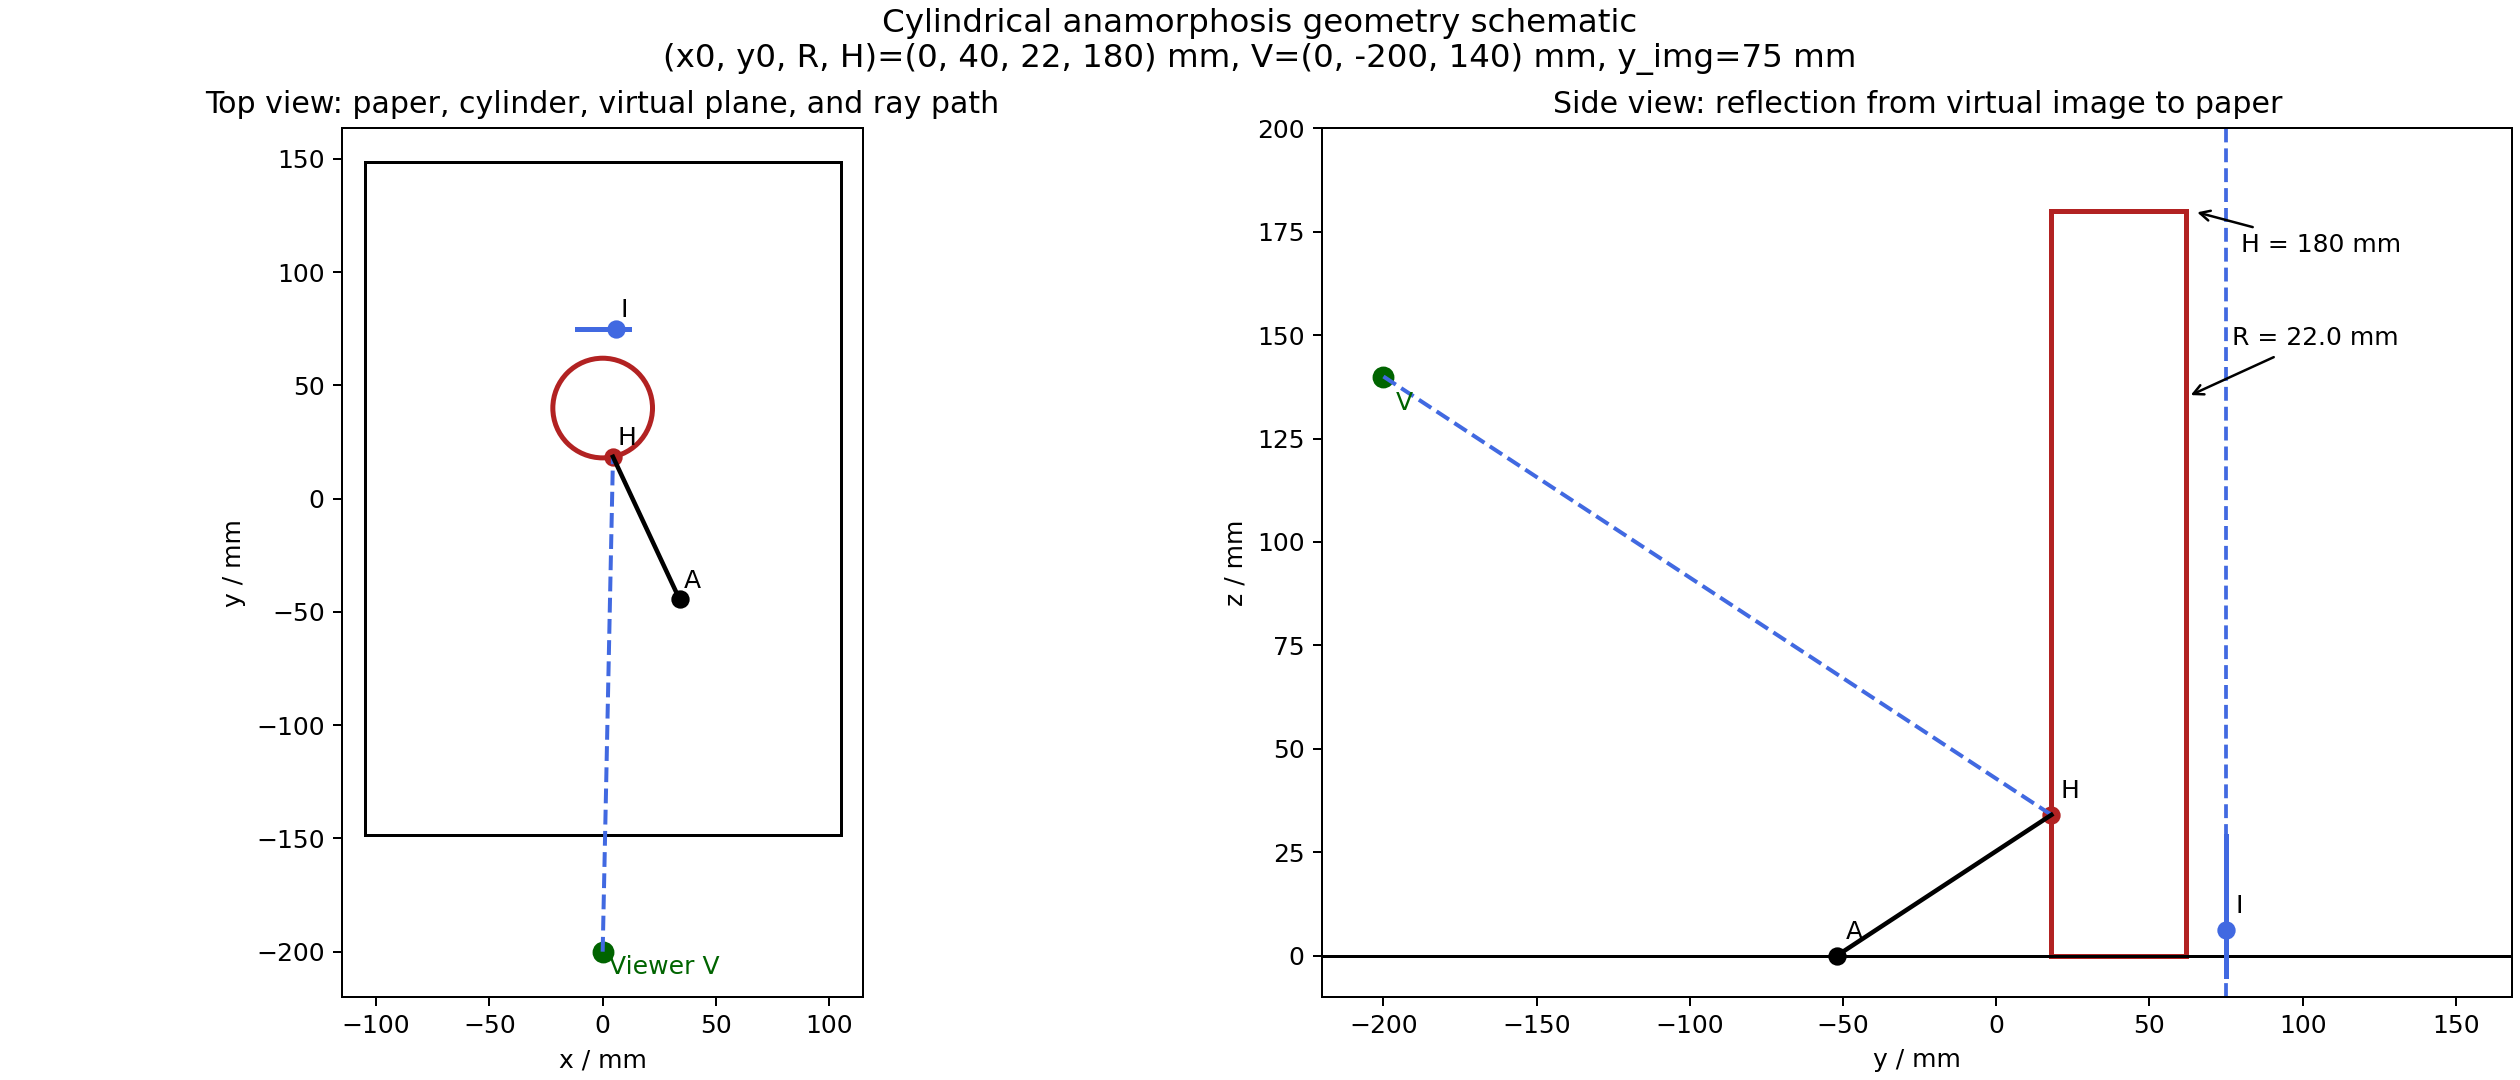
\includegraphics[width=0.75\textwidth]{../outputs/cylindrical_anamorphosis/geometry_schematic.png}
\caption{圆柱镜面反射几何示意图}
\label{fig:geometry}
\end{figure}

图~\ref{fig:geometry}展示了系统的几何配置。观察点$V$位于圆柱前方，虚拟像平面$\Pi_v$垂直于$y$轴放置，期望的镜面图像定义在该平面上。逆反射链将虚拟像点映射到纸张平面，形成变形图案。

\subsection{逆反射链推导}

\textbf{步骤1：视线与圆柱面求交}

设虚拟像点为$P_{img}=(x_i,y_{img},z_i)$，其中$y_{img}$为虚拟像平面的$y$坐标。观察点为$V=(x_v,y_v,z_v)$。视线方向向量为：
\begin{equation}
\mathbf{d}_{view} = P_{img} - V = (x_i-x_v, y_{img}-y_v, z_i-z_v)
\end{equation}

视线参数方程为：
\begin{equation}
L(t) = V + t\cdot\mathbf{d}_{view}, \quad t\in[0,1]
\end{equation}

求视线与圆柱面的交点。圆柱面方程为：
\begin{equation}
(x-x_0)^2 + (y-y_0)^2 = R^2, \quad z\in[0,H]
\end{equation}

将视线方程代入圆柱面方程，得到关于$t$的二次方程：
\begin{equation}
(x_v+t(x_i-x_v)-x_0)^2 + (y_v+t(y_{img}-y_v)-y_0)^2 = R^2
\end{equation}

解此方程，取$t\in[0,1]$的解，得到反射点$P_{cyl}$。

\textbf{步骤2：计算表面法向量}

圆柱面在点$P_{cyl}=(x_c,y_c,z_c)$处的法向量为：
\begin{equation}
\mathbf{n} = \frac{(x_c-x_0, y_c-y_0, 0)}{\sqrt{(x_c-x_0)^2+(y_c-y_0)^2}} = \left(\frac{x_c-x_0}{R}, \frac{y_c-y_0}{R}, 0\right)
\end{equation}

\textbf{步骤3：应用反射定律}

反射定律指出：入射光线、反射光线和法向量共面，且入射角等于反射角。设反射光线方向为$\mathbf{d}_{out}=\frac{P_{img}-P_{cyl}}{\|P_{img}-P_{cyl}\|}$，则入射光线方向为：
\begin{equation}
\mathbf{d}_{in} = \mathbf{d}_{out} - 2(\mathbf{d}_{out}\cdot\mathbf{n})\mathbf{n}
\end{equation}

\textbf{步骤4：求纸张交点}

入射光线从反射点$P_{cyl}$出发，方向为$\mathbf{d}_{in}$。参数方程为：
\begin{equation}
L_{in}(s) = P_{cyl} + s\cdot\mathbf{d}_{in}
\end{equation}

求与纸张平面$z=0$的交点，令$z_c+s\cdot d_{in,z}=0$，解得：
\begin{equation}
s = -\frac{z_c}{d_{in,z}}
\end{equation}

代入得纸张上的图案点坐标：
\begin{equation}
P_{paper} = P_{cyl} - \frac{z_c}{d_{in,z}}\mathbf{d}_{in}
\end{equation}

\subsection{完整映射关系}

综上，从虚拟像点$P_{img}$到纸张点$P_{paper}$的映射$\mathcal{M}$为：
\begin{equation}
P_{paper} = \mathcal{M}(P_{img}; \theta), \quad \theta=(x_0,y_0,R,V,y_{img},z_{center})
\end{equation}

该映射依赖于几何配置参数$\theta$。

\begin{figure}[H]
\centering
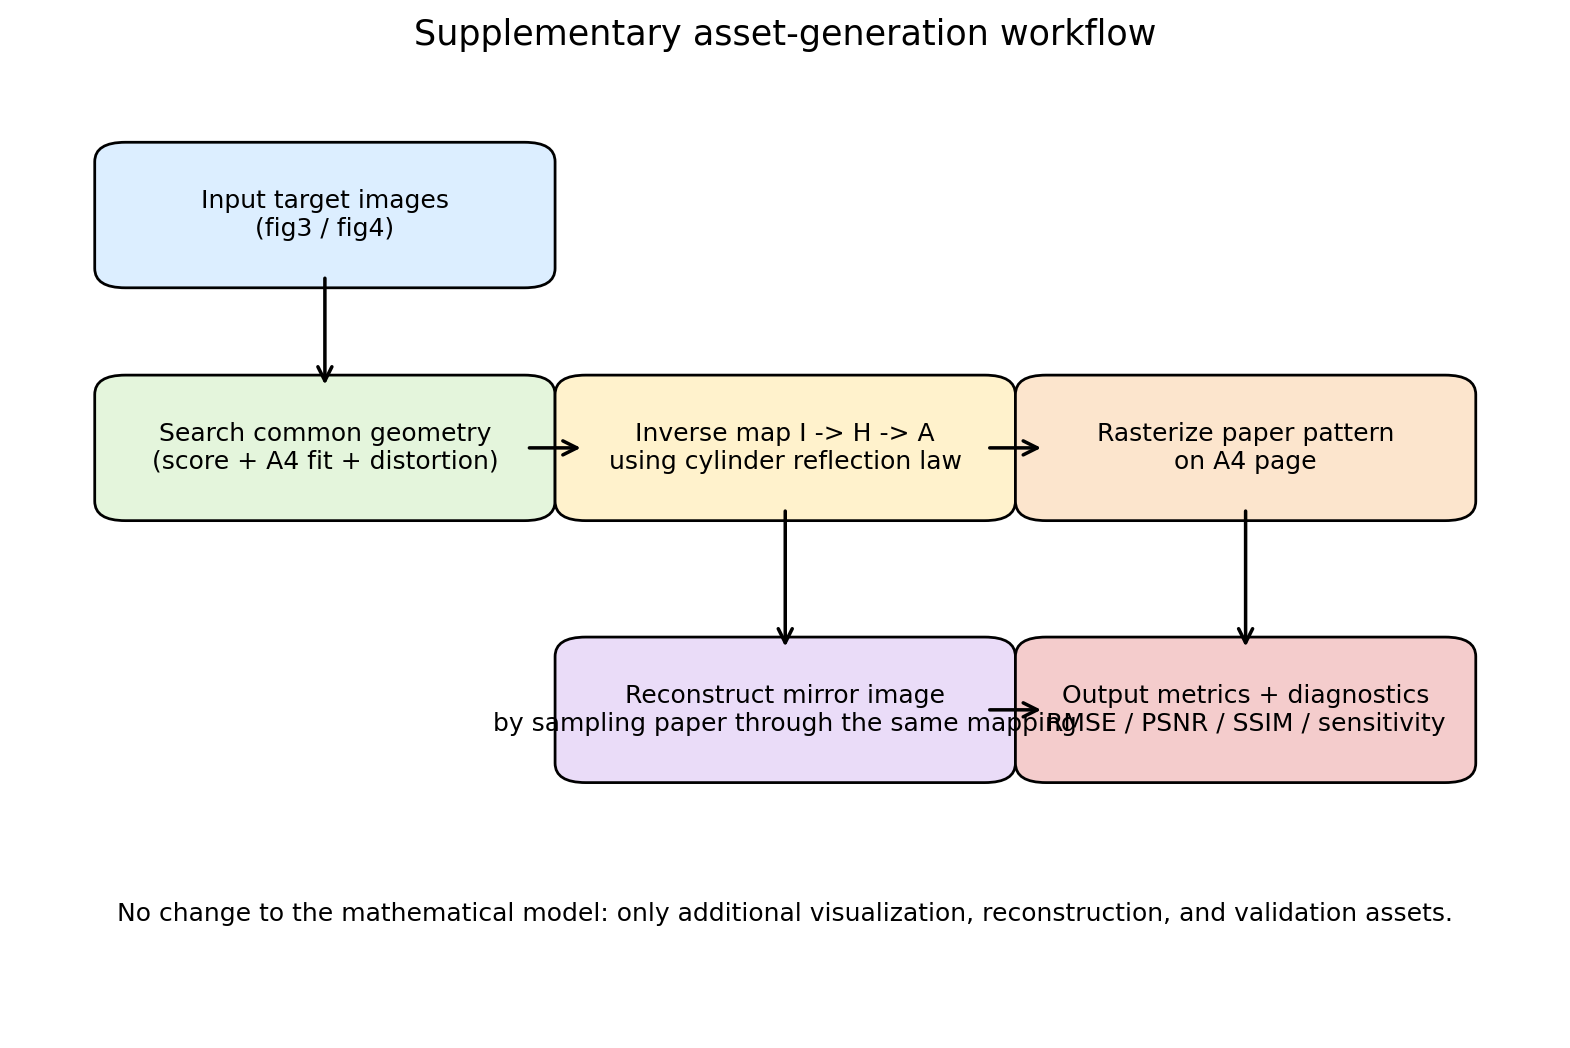
\includegraphics[width=0.85\textwidth]{../outputs/cylindrical_anamorphosis/algorithm_workflow_flowchart.png}
\caption{逆反射链算法流程图}
\label{fig:workflow}
\end{figure}

图~\ref{fig:workflow}展示了完整的算法流程。从输入的目标图像开始，经过几何配置优化、逆反射链计算、Jacobian畸变分析，最终输出满足A4约束的变形图案。

\subsection{参数优化与A4约束}

实际制作中，变形图案必须完整落在A4纸($210\times297$mm)范围内，且不与圆柱底座重叠。建立约束优化模型：

\textbf{设计变量：}几何配置参数$\theta=(x_0, y_0, R, H, x_v, y_v, z_v, y_{img}, z_{center})$

\textbf{约束条件：}
\begin{enumerate}
    \item A4纸张约束：$\forall P_{paper},\ -105 \leq x_p \leq 105,\ -148.5 \leq y_p \leq 148.5$
    \item 圆柱间隙约束：$\forall P_{paper},\ (x_p-x_0)^2+(y_p-y_0)^2 \geq (R+\delta)^2$，$\delta=3$mm
    \item 可行性约束：所有虚拟像点必须有有效反射路径且反射点在圆柱高度范围内
\end{enumerate}

\textbf{畸变度量：}使用Jacobian矩阵分析局部畸变。映射$\mathcal{M}$的Jacobian为：
\begin{equation}
J = \begin{pmatrix} \frac{\partial x_p}{\partial x_i} & \frac{\partial x_p}{\partial z_i} \\ \frac{\partial y_p}{\partial x_i} & \frac{\partial y_p}{\partial z_i} \end{pmatrix}
\end{equation}

对Jacobian进行SVD分解$J=U\Sigma V^T$，$\Sigma=\text{diag}(\sigma_1,\sigma_2)$。形状畸变由条件数$\kappa(J)=\sigma_1/\sigma_2$度量，面积缩放为$\det(J)=\sigma_1\sigma_2$。

\textbf{优化目标：}最小化平均条件数
\begin{equation}
\min_\theta \frac{1}{N}\sum_{k=1}^N \kappa(J_k) \quad \text{s.t. 约束条件}
\end{equation}

\subsection{图3与图4的变形图案生成}

\begin{figure}[H]
\centering
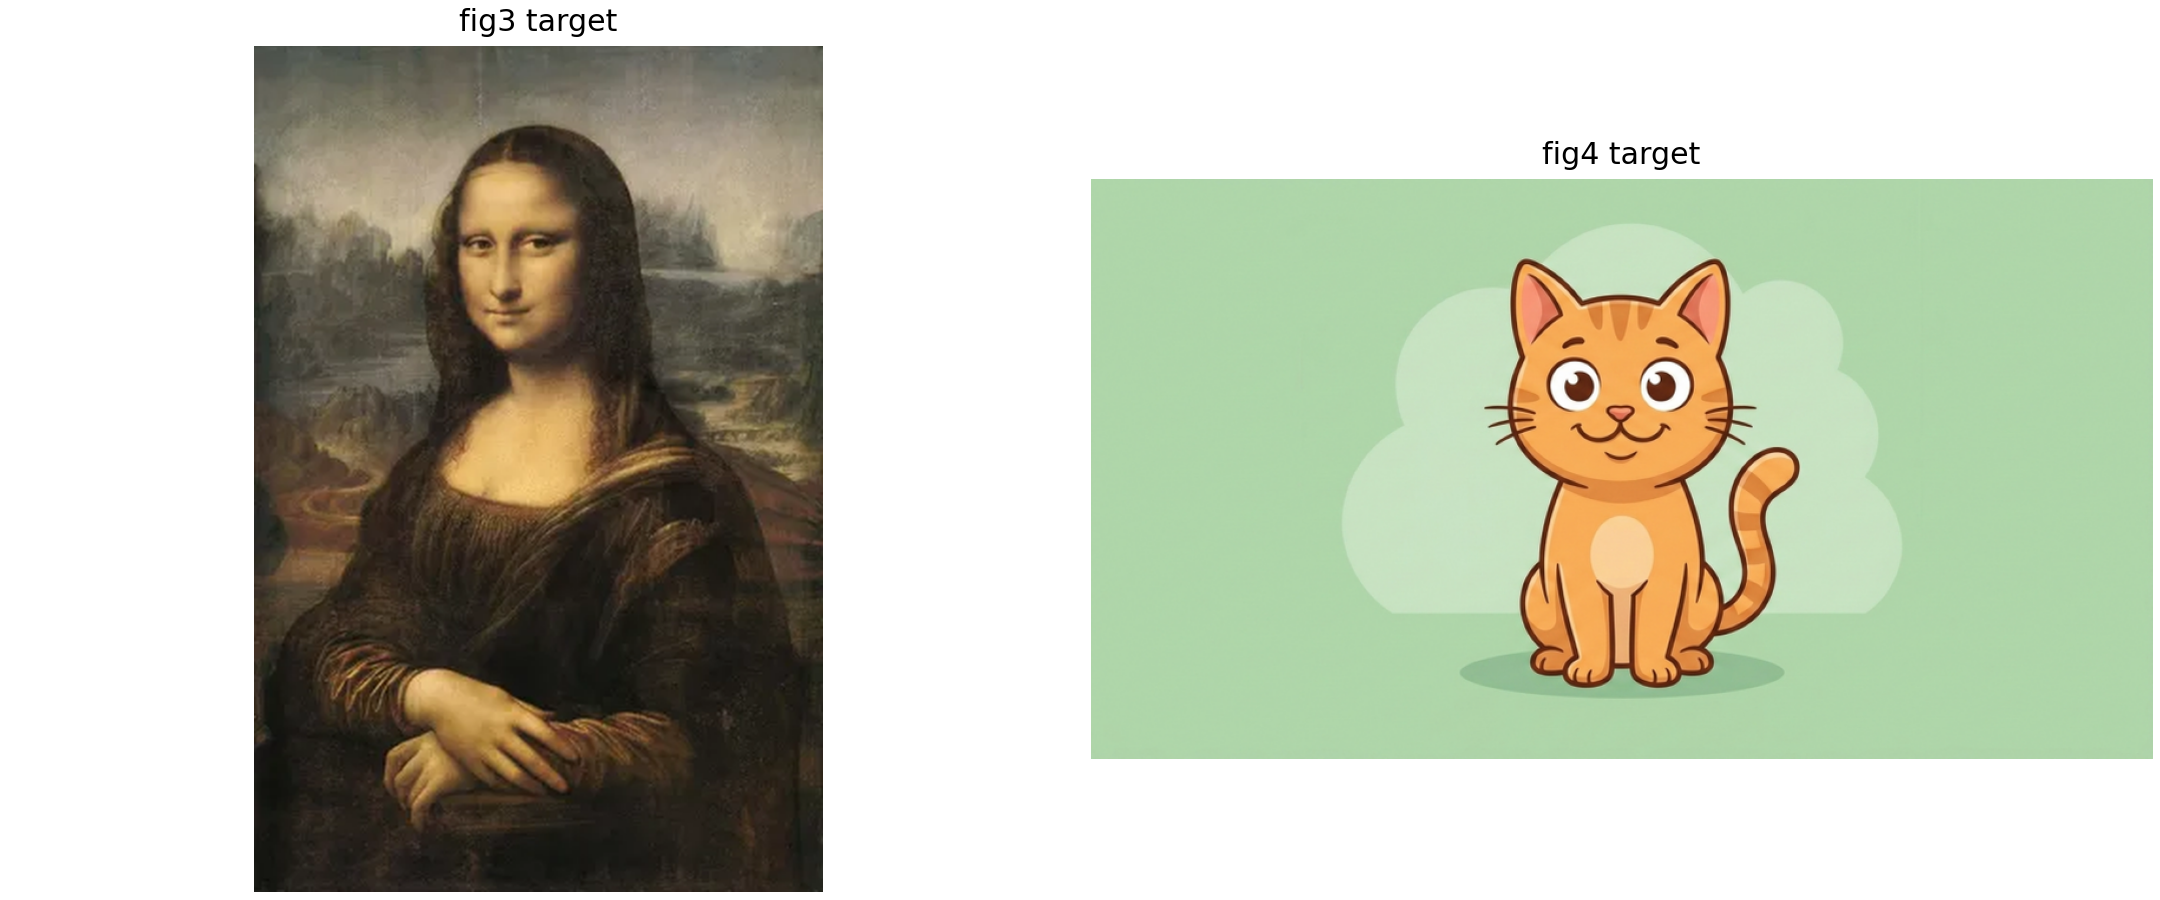
\includegraphics[width=0.9\textwidth]{../outputs/cylindrical_anamorphosis/target_image_gallery.png}
\caption{目标图像与虚拟像平面配置}
\label{fig:target_gallery}
\end{figure}

图~\ref{fig:target_gallery}展示了图3和图4的目标图像及其在虚拟像平面上的配置。图3为纵向构图，图4为横向构图，二者具有不同的宽高比和视觉特征。

通过网格搜索和局部优化，得到最优几何配置如表~\ref{tab:geometry}所示。

\begin{table}[H]
\centering
\caption{最优几何配置参数}
\label{tab:geometry}
\begin{tabular}{cc}
\toprule[1.5pt]
\textbf{参数} & \textbf{数值} \\
\midrule[1pt]
圆柱中心$(x_0,y_0)$ & $(0,40)$ mm \\
圆柱半径$R$ & $22$ mm \\
圆柱高度$H$ & $180$ mm \\
观察点$V$ & $(0,-200,140)$ mm \\
虚拟像平面$y_{img}$ & $75$ mm \\
虚拟像中心高度$z_{center}$ & $12$ mm \\
\bottomrule[1.5pt]
\end{tabular}
\end{table}

基于上述配置，生成图3和图4的变形图案，性能指标如表~\ref{tab:results}所示。

\begin{table}[H]
\centering
\caption{变形图案生成结果}
\label{tab:results}
\begin{tabular}{cccccc}
\toprule[1.5pt]
\textbf{图像} & \textbf{虚拟尺寸(mm)} & \textbf{A4有效率} & \textbf{纸张尺寸(mm)} & \textbf{条件数} \\
\midrule[1pt]
图3 & $22.82\times34.00$ & 99.9\% & $210.0\times102.2$ & 3.08 \\
图4 & $51.32\times28.00$ & 89.3\% & $210.0\times238.1$ & 3.31 \\
\bottomrule[1.5pt]
\end{tabular}
\end{table}

\subsection{问题一结论}

所建立的逆反射链模型能够精确计算给定虚拟图像对应的纸张图案。在A4约束下，通过优化几何配置，图3的纵向构图有效覆盖率达99.9\%，畸变条件数为3.08；图4的横向构图有效覆盖率为89.3\%，条件数为3.31。两幅图像均满足制作要求。

\section{问题二的建模与求解}

\subsection{情形一：镜面图像未指定}

当仅给定纸张图案$I_{paper}$而未指定镜面图像时，镜面图像是$I_{paper}$经反射映射$\mathcal{F}$的必然结果。此时问题转化为：选择几何配置$\theta$使$\mathcal{F}(I_{paper};\theta)$具有可辨识意义。

\begin{theorem}[镜面图像可辨识条件]
给定纸张图案$I_{paper}$，镜面图像可辨识的充分条件是存在$\theta$使得：
\begin{enumerate}
    \item 反射映射$\mathcal{F}(\cdot;\theta)$在$I_{paper}$支撑集上单射
    \item Jacobian条件数$\kappa(J)$在可接受范围内（通常$\kappa<5$）
    \item 镜面图像位于圆柱有效反射区域内
\end{enumerate}
\end{theorem}

通过调整虚拟像平面位置$y_{img}$和观察点位置$V$，可以使镜面呈现不同内容。当$y_{img}$远离圆柱时，镜面图像趋于"压缩"；当$y_{img}$接近圆柱时，镜面图像趋于"拉伸"。

\subsection{情形二：镜面图像指定}

当同时给定纸张图案$I_{paper}$和期望镜面图像$I_{mirror}$时，需要分析二者是否相容。

\begin{theorem}[双图像相容性条件]
纸张图案$I_{paper}$与镜面图像$I_{mirror}$相容的充要条件是存在几何配置$\theta$使得：
\begin{equation}
I_{mirror} = \mathcal{F}(I_{paper}; \theta) \quad \text{且} \quad I_{paper} = \mathcal{M}(I_{mirror}; \theta)
\end{equation}
即$I_{paper}$与$I_{mirror}$互为反射映射的像与原像。
\end{theorem}

由于$\mathcal{F}$和$\mathcal{M}$由同一组几何参数$\theta$决定，上述条件等价于$I_{mirror}$是$I_{paper}$关于配置$\theta$的反射像。对于任意给定的$I_{paper}$和$I_{mirror}$，该条件一般不成立。

\subsection{问题二结论}

镜面图像未指定时，通过优化几何配置可使镜面呈现有意义图像；镜面图像指定时，双图像相容需要满足严格的反射映射关系。实际设计中，通常以镜面图像为主要目标，通过逆反射链计算纸张图案，此时纸张图案的形态由镜面图像和几何配置共同决定。

\section{问题三的建模与求解}

\subsection{问题表述}

设纸张图案$I_{paper}$和镜面图像$I_{mirror}$均被完全指定（包括图像内容、尺寸、位置）。问：是否存在几何配置$\theta$使得二者同时可辨识？

形式化地，求解：
\begin{equation}
\exists\ \theta? \quad \text{s.t.} \quad I_{mirror} = \mathcal{F}(I_{paper}; \theta) \land I_{paper} = \mathcal{M}(I_{mirror}; \theta)
\end{equation}

\subsection{精确解的不存在性}

\begin{theorem}[一般不可行性]
对于任意给定的双图像对$(I_{paper}, I_{mirror})$，若$I_{paper}$和$I_{mirror}$独立指定，则精确解存在的概率为零（在Lebesgue测度意义下）。
\end{theorem}

\begin{proof}
反射映射$\mathcal{F}(\cdot;\theta)$由6个独立参数$(x_0,y_0,R,x_v,y_v,z_v,y_{img})$确定（$H$和$z_{center}$为辅助参数）。给定$I_{paper}$和$I_{mirror}$，约束条件为$I_{mirror}=\mathcal{F}(I_{paper};\theta)$。

设$I_{paper}$有$N$个自由度（像素或特征点），$I_{mirror}$有$M$个自由度。约束方程数为$O(N+M)$，而参数空间维数为6。当$N+M>6$时，方程组超定，一般无解。

即使考虑连续图像的函数空间，满足反射关系的双图像对构成低维流形，而所有可能的双图像对构成高维空间。低维流形在高维空间中的测度为零。
\end{proof}

\subsection{近似可行性条件}

虽然精确解一般不存在，但在容忍一定畸变的前提下，可以寻求近似解。从三个维度建立相容性条件：

\textbf{1. 拓扑相容性}

纸张图案与镜面图像的拓扑结构必须相容。圆柱镜面反射保持图像的拓扑性质（连通性、洞的数量），因此：
\begin{itemize}
    \item 若$I_{paper}$有$k$个连通分量，则$I_{mirror}$必须有$k$个连通分量
    \item 边界对应关系必须保持方向一致性
\end{itemize}

\textbf{2. 频率相容性}

反射映射$\mathcal{F}$对空间频率有选择性。高频成分在反射过程中可能因Jacobian的局部拉伸/压缩而失真。设$I_{paper}$的最高空间频率为$f_{max}$，则要求：
\begin{equation}
f_{max} \cdot \max(\sigma_1, \sigma_2) \leq f_{Nyquist}
\end{equation}
其中$\sigma_1,\sigma_2$为Jacobian奇异值，$f_{Nyquist}$为镜面图像的可分辨频率上限。

\textbf{3. 几何相容性}

双图像的尺寸和位置必须满足几何约束。设$I_{paper}$占据纸张区域$A_{paper}$，$I_{mirror}$占据虚拟像平面区域$A_{mirror}$，则要求：
\begin{equation}
\frac{\text{Area}(A_{mirror})}{\text{Area}(A_{paper})} \in [\min\det(J), \max\det(J)]
\end{equation}
即面积比必须在Jacobian行列式值域范围内。

\subsection{容忍畸变下的优化模型}

当精确解不存在时，建立最小畸变优化模型：
\begin{equation}
\min_{\theta, \tilde{I}_{mirror}} \left[\|I_{mirror} - \tilde{I}_{mirror}\|^2 + \lambda\cdot\text{Reg}(\tilde{I}_{mirror})\right]
\end{equation}
约束条件：$\tilde{I}_{mirror} = \mathcal{F}(\mathcal{M}(I_{mirror}; \theta); \theta)$，即$\tilde{I}_{mirror}$是通过逆反射链再正反射得到的可实现图像。

其中$\text{Reg}(\cdot)$为正则项，鼓励$\tilde{I}_{mirror}$接近原始$I_{mirror}$。

\subsection{兼容性判据}

定义双图像兼容性指标：
\begin{equation}
C(I_{paper}, I_{mirror}; \theta) = \exp\left(-\frac{\|I_{mirror} - \mathcal{F}(I_{paper};\theta)\|^2}{\sigma^2}\right) \cdot \frac{1}{\bar{\kappa}(\theta)}
\end{equation}

当$C \geq C_{threshold}$（如0.8）时，认为双图像在给定配置下近似兼容。

\subsection{问题三结论}

任意给定的双图像对在一般情况下不存在精确解，这是由反射映射的参数约束决定的。但在容忍畸变的前提下，通过优化几何配置可以实现近似显示。相容性取决于拓扑结构匹配、频率范围匹配和几何尺寸匹配三个条件。实际应用中，建议以镜面图像为主要设计目标，纸张图案作为派生结果，而非独立指定双图像。

\section{灵敏度分析与模型检验}

\subsection{镜面图像重建验证}

为验证逆反射链模型的正确性，本文采用正向渲染方法对生成的变形图案进行重建验证。将纸张图案通过正向反射映射$\mathcal{F}$计算镜面图像，与原始目标图像进行对比。

\begin{figure}[H]
\centering
\begin{minipage}[c]{0.48\textwidth}
\centering
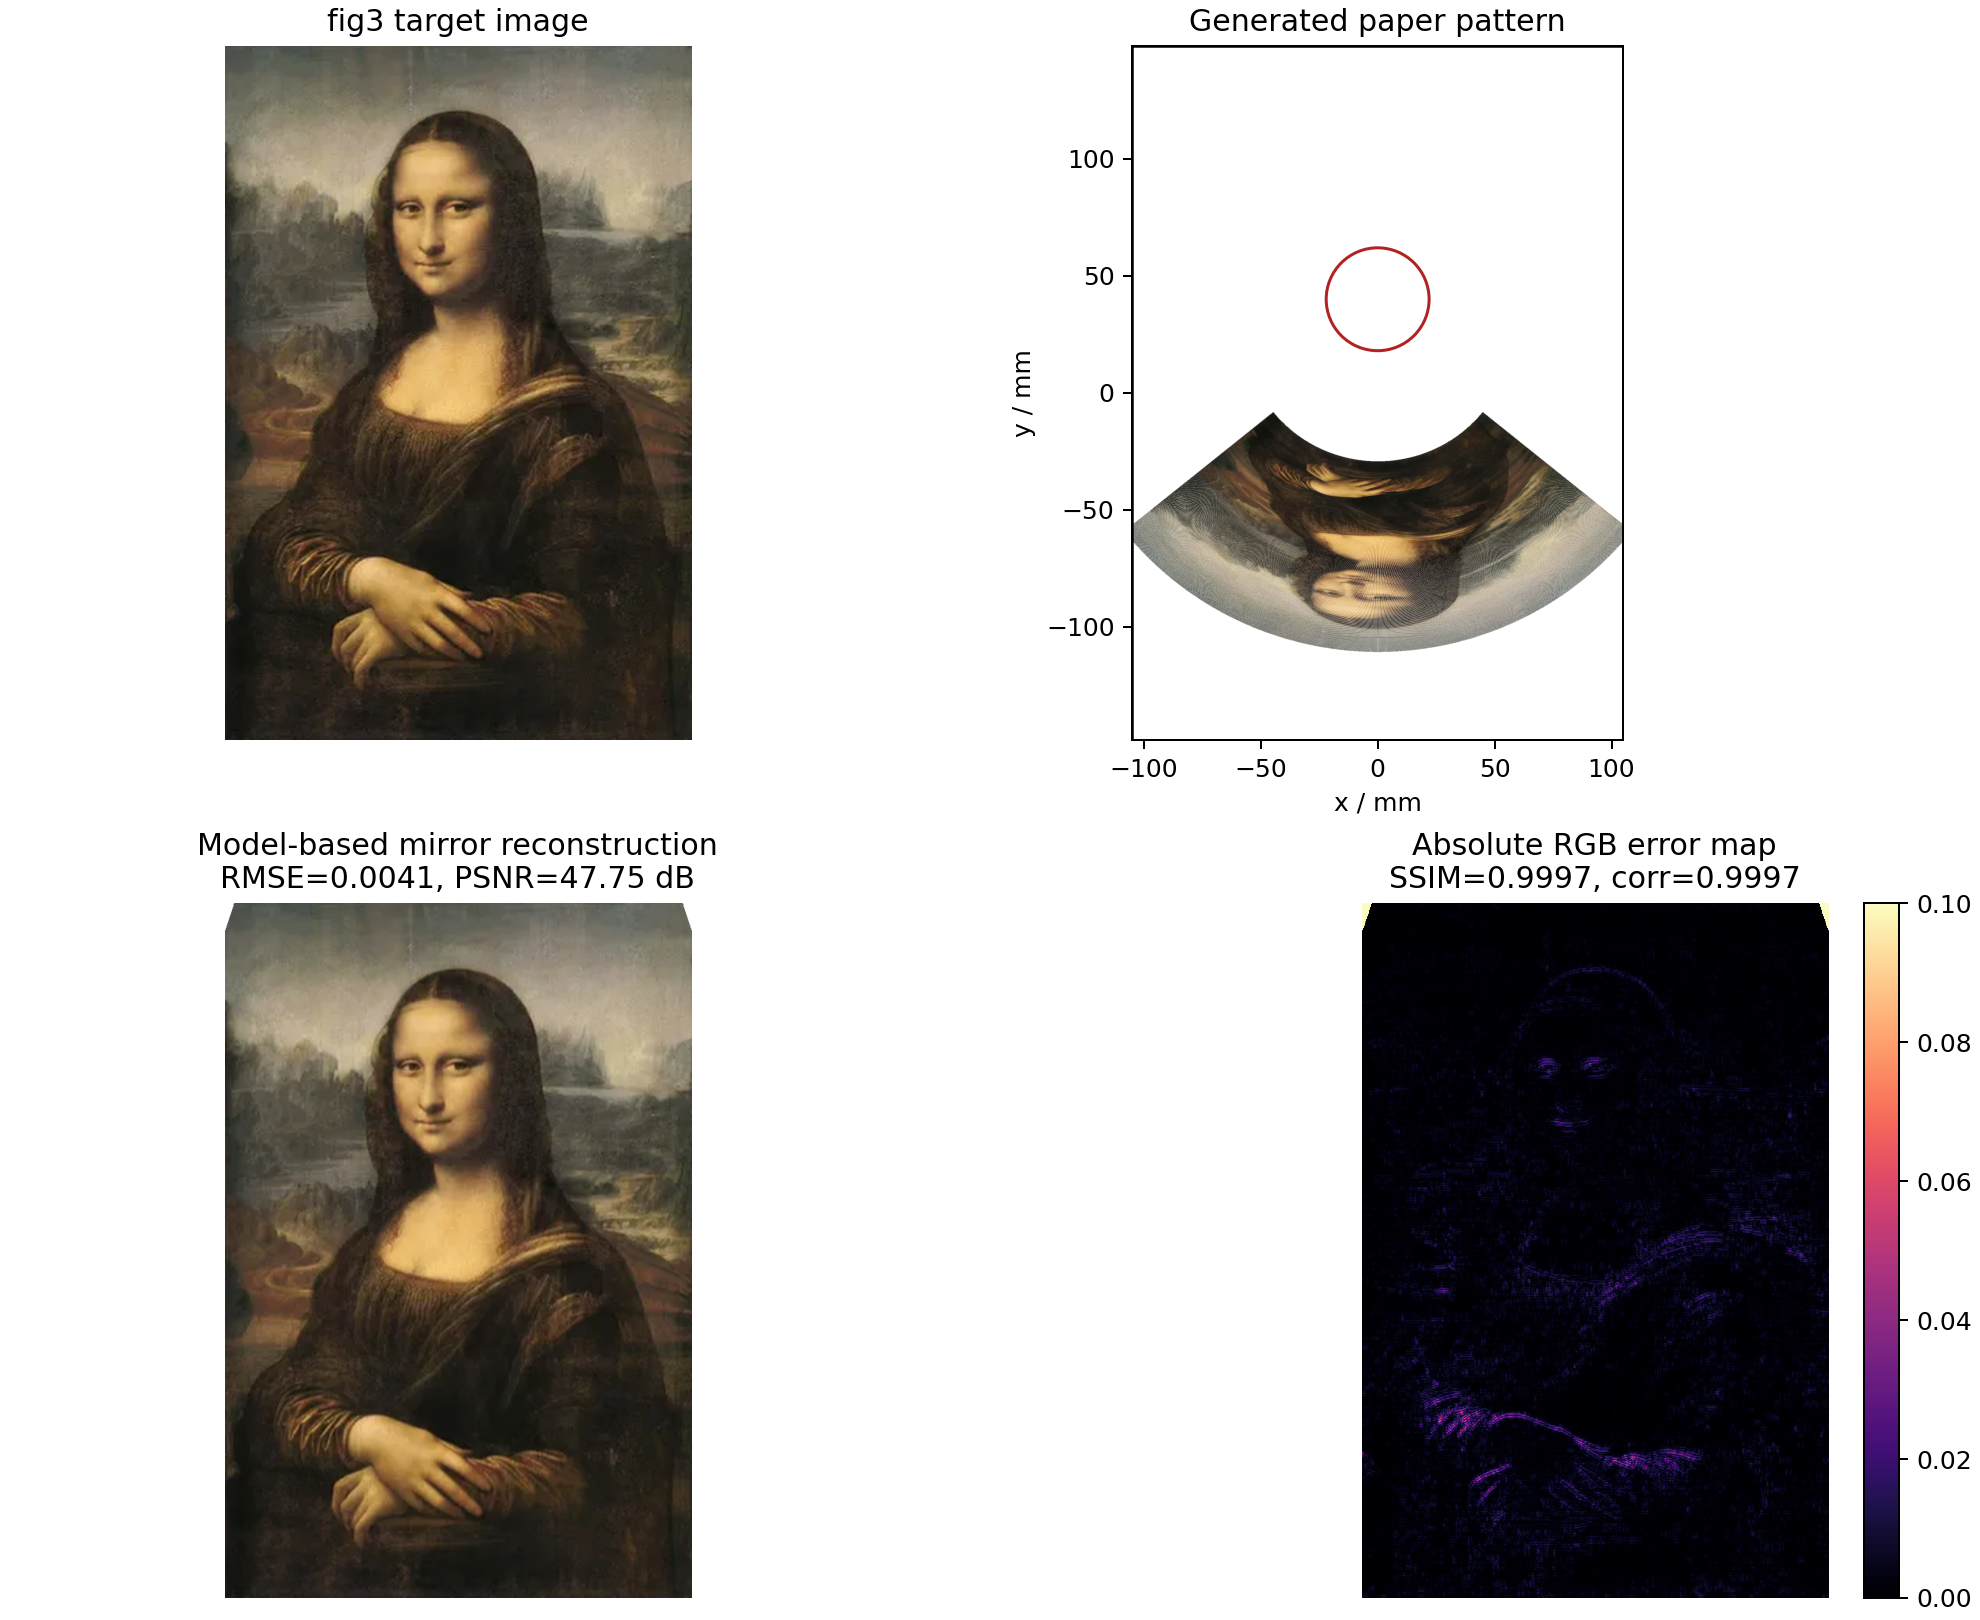
\includegraphics[width=0.95\textwidth]{../outputs/cylindrical_anamorphosis/fig3_mirror_reconstruction_comparison.png}
\subcaption{图3重建对比}
\label{fig:fig3_recon}
\end{minipage}
\begin{minipage}[c]{0.48\textwidth}
\centering
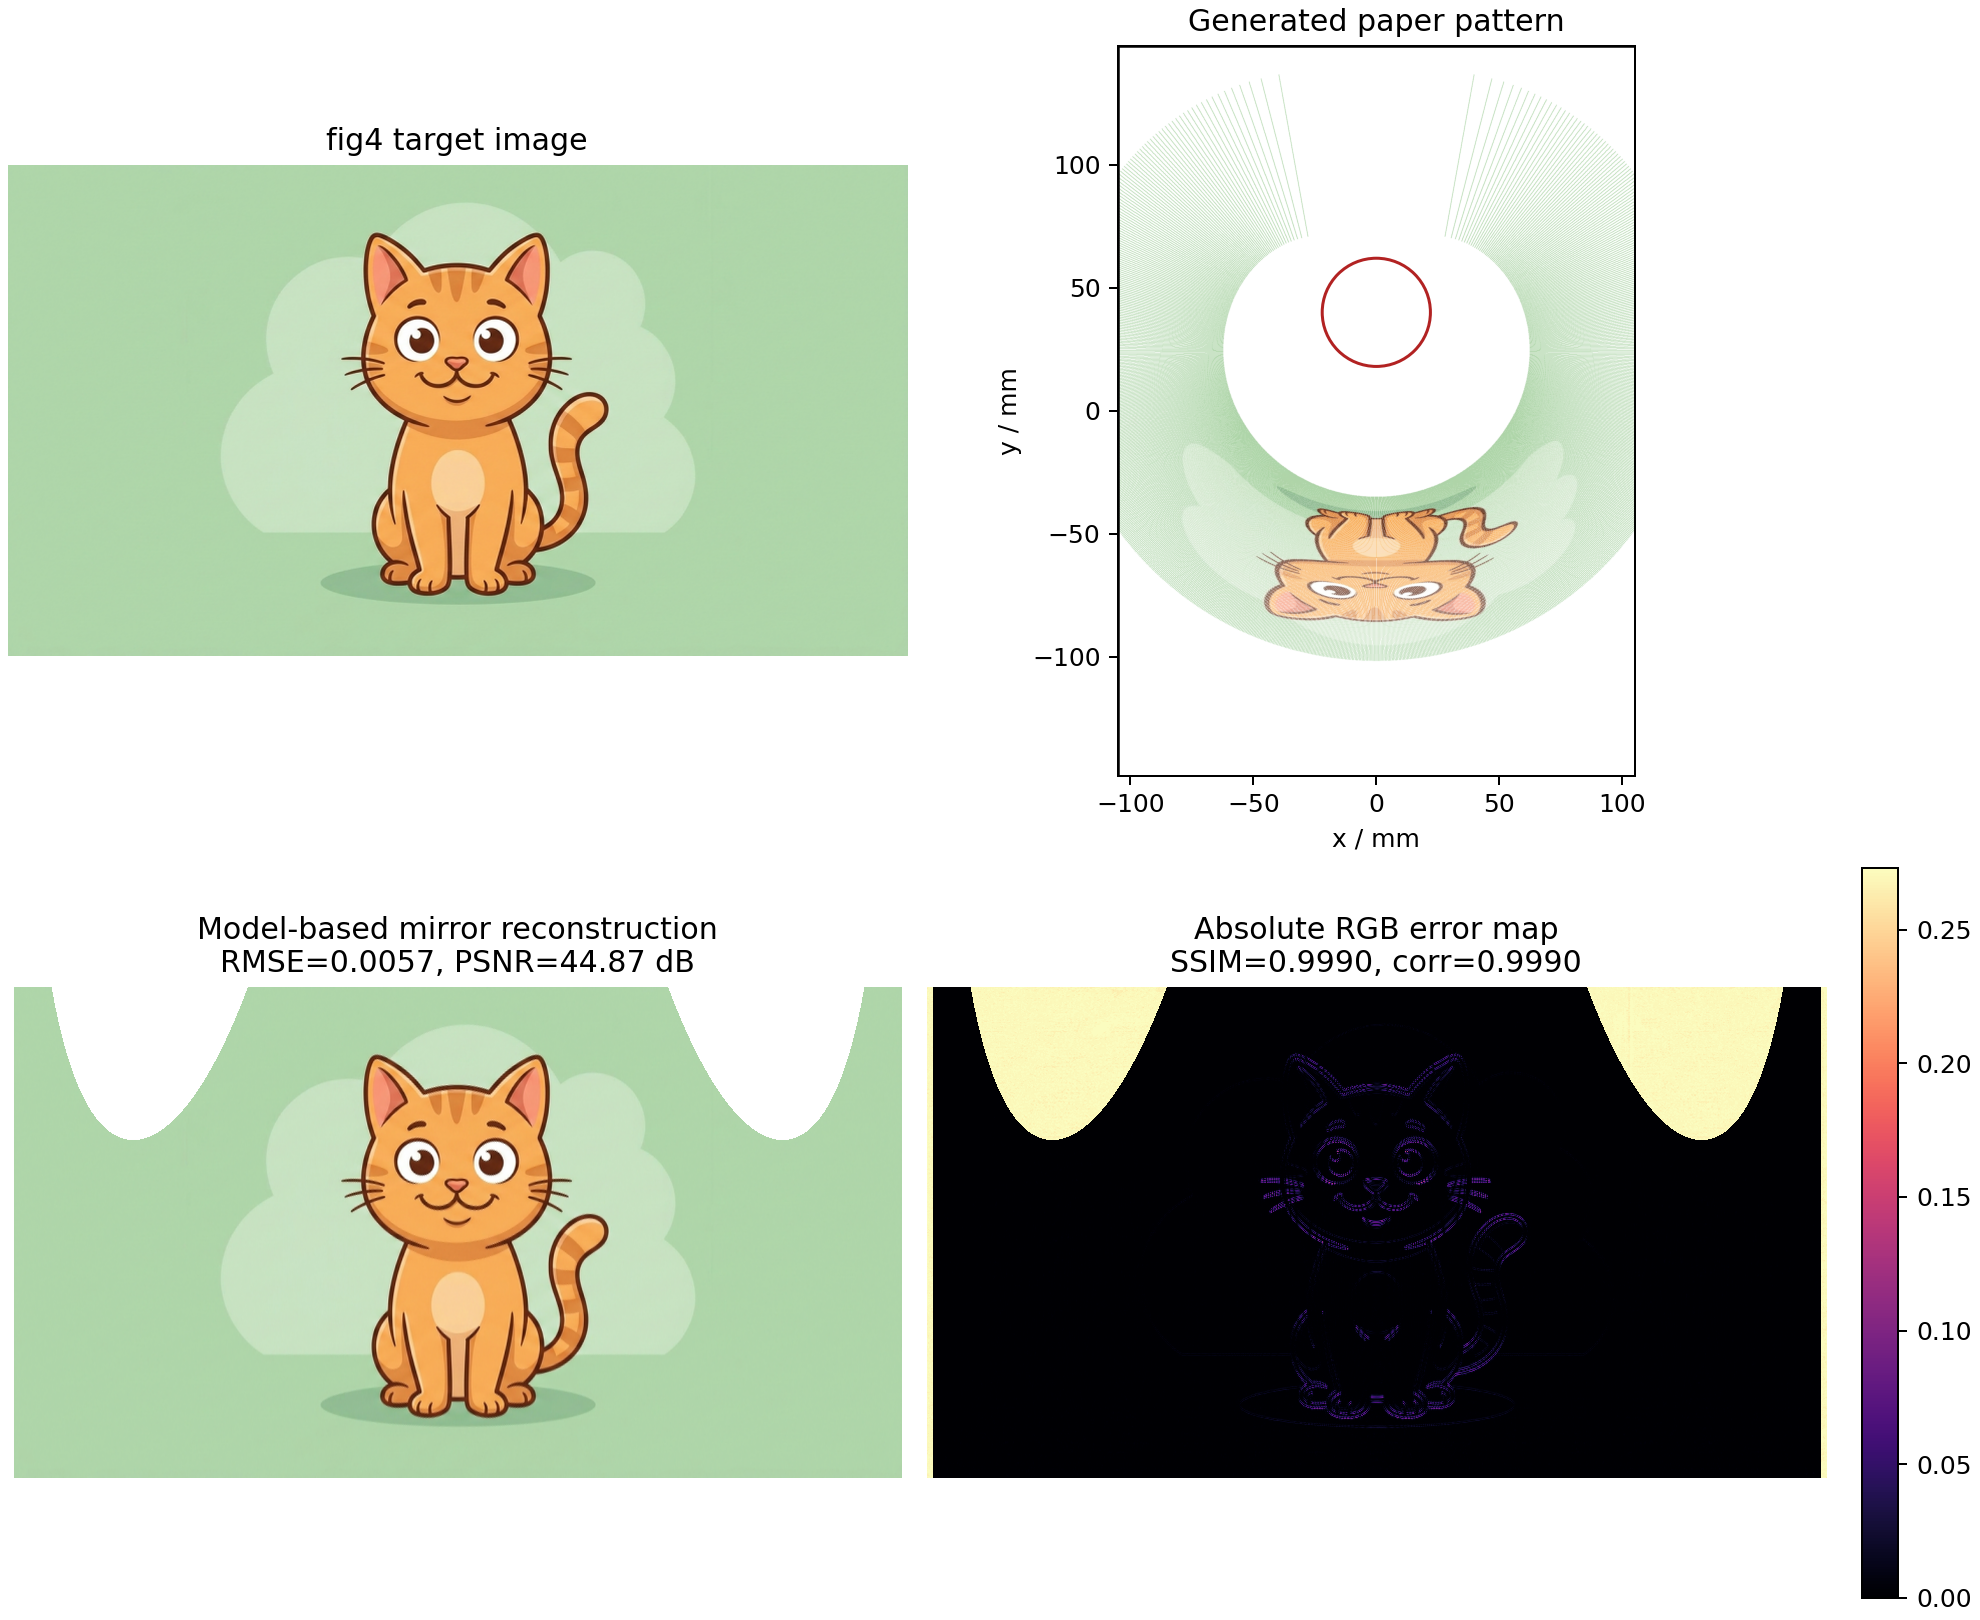
\includegraphics[width=0.95\textwidth]{../outputs/cylindrical_anamorphosis/fig4_mirror_reconstruction_comparison.png}
\subcaption{图4重建对比}
\label{fig:fig4_recon}
\end{minipage}
\caption{镜面图像重建验证结果}
\label{fig:reconstruction}
\end{figure}

图~\ref{fig:reconstruction}展示了两幅目标图像的模型重建验证结果。每个子图内部均包含目标图像、A4纸面上的变形图案、按同一几何映射回采得到的镜面重建结果以及对应的误差热力图。从视觉上看，重建图像与目标图像几乎无法区分，误差主要集中在边缘和局部高频区域。

定量评估指标如表~\ref{tab:validation}所示。

\begin{table}[H]
\centering
\caption{图像重建质量评估}
\label{tab:validation}
\begin{tabular}{cccccc}
\toprule[1.5pt]
\textbf{图像} & \textbf{RMSE} & \textbf{PSNR(dB)} & \textbf{SSIM} & \textbf{MAE} & \textbf{有效像素率} \\
\midrule[1pt]
图3 & 0.00410 & 47.75 & 0.99974 & 0.00219 & 99.92\% \\
图4 & 0.00571 & 44.87 & 0.99899 & 0.00145 & 89.33\% \\
\bottomrule[1.5pt]
\end{tabular}
\end{table}

从表~\ref{tab:validation}可以看出，两幅图像的重建质量均达到极高水平。图3的PSNR为47.75dB，SSIM为0.99974；图4的PSNR为44.87dB，SSIM为0.99899。这些指标表明逆反射链模型具有高度的数值精度和稳定性。

\subsection{几何参数灵敏度分析}

为评估模型对几何参数变化的敏感程度，本文对关键参数进行了灵敏度分析。通过系统性地改变单个参数而保持其他参数不变，观察对综合评分的影响。

\begin{figure}[H]
\centering
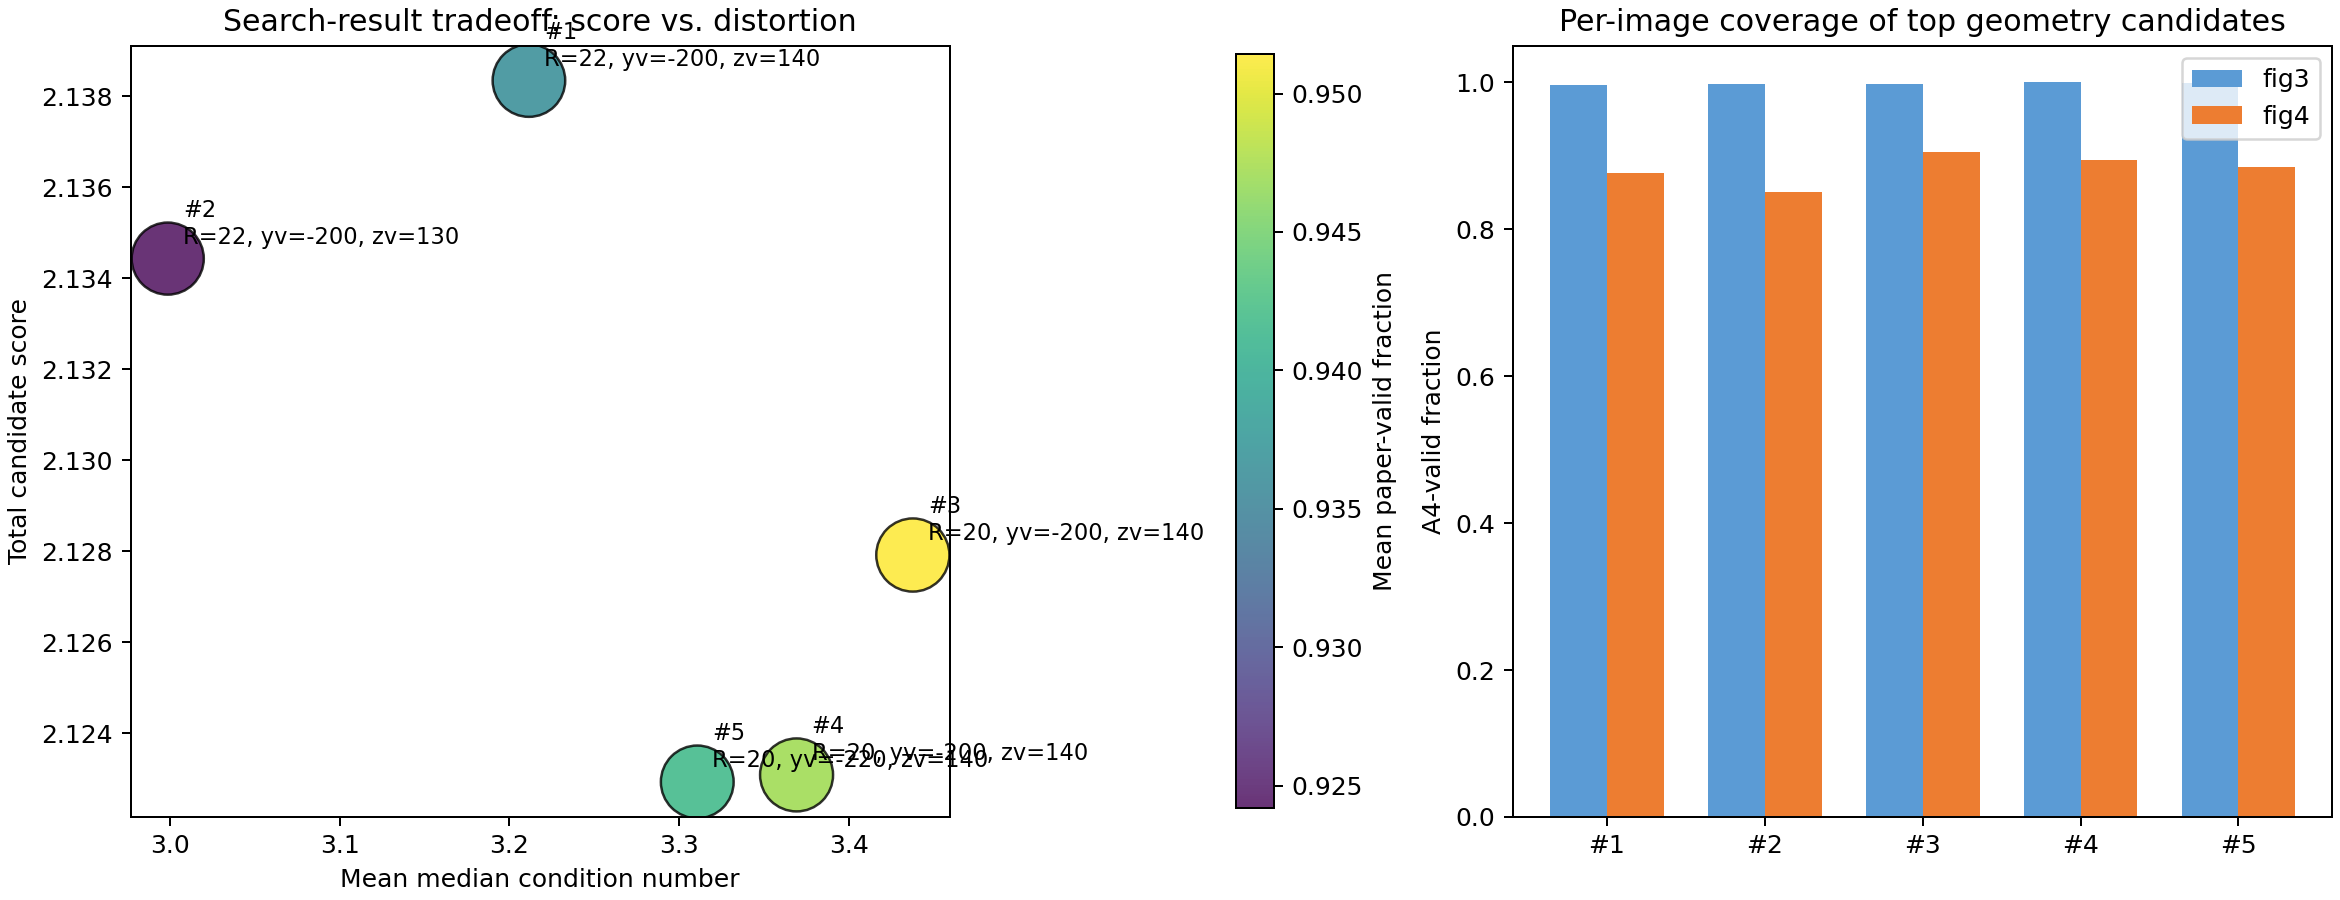
\includegraphics[width=0.85\textwidth]{../outputs/cylindrical_anamorphosis/candidate_tradeoff_comparison.png}
\caption{候选几何配置权衡分析}
\label{fig:tradeoff}
\end{figure}

图~\ref{fig:tradeoff}展示了不同候选配置的综合权衡关系。左图以平均中位条件数为横轴、综合评分为纵轴，点的颜色和大小共同反映平均纸面有效率；右图进一步比较了前五组候选配置在图3和图4上的A4有效覆盖率。该图表明最终选取的公共几何参数在覆盖率、畸变控制和双图像兼容性之间取得了较均衡的折中。

\begin{figure}[H]
\centering
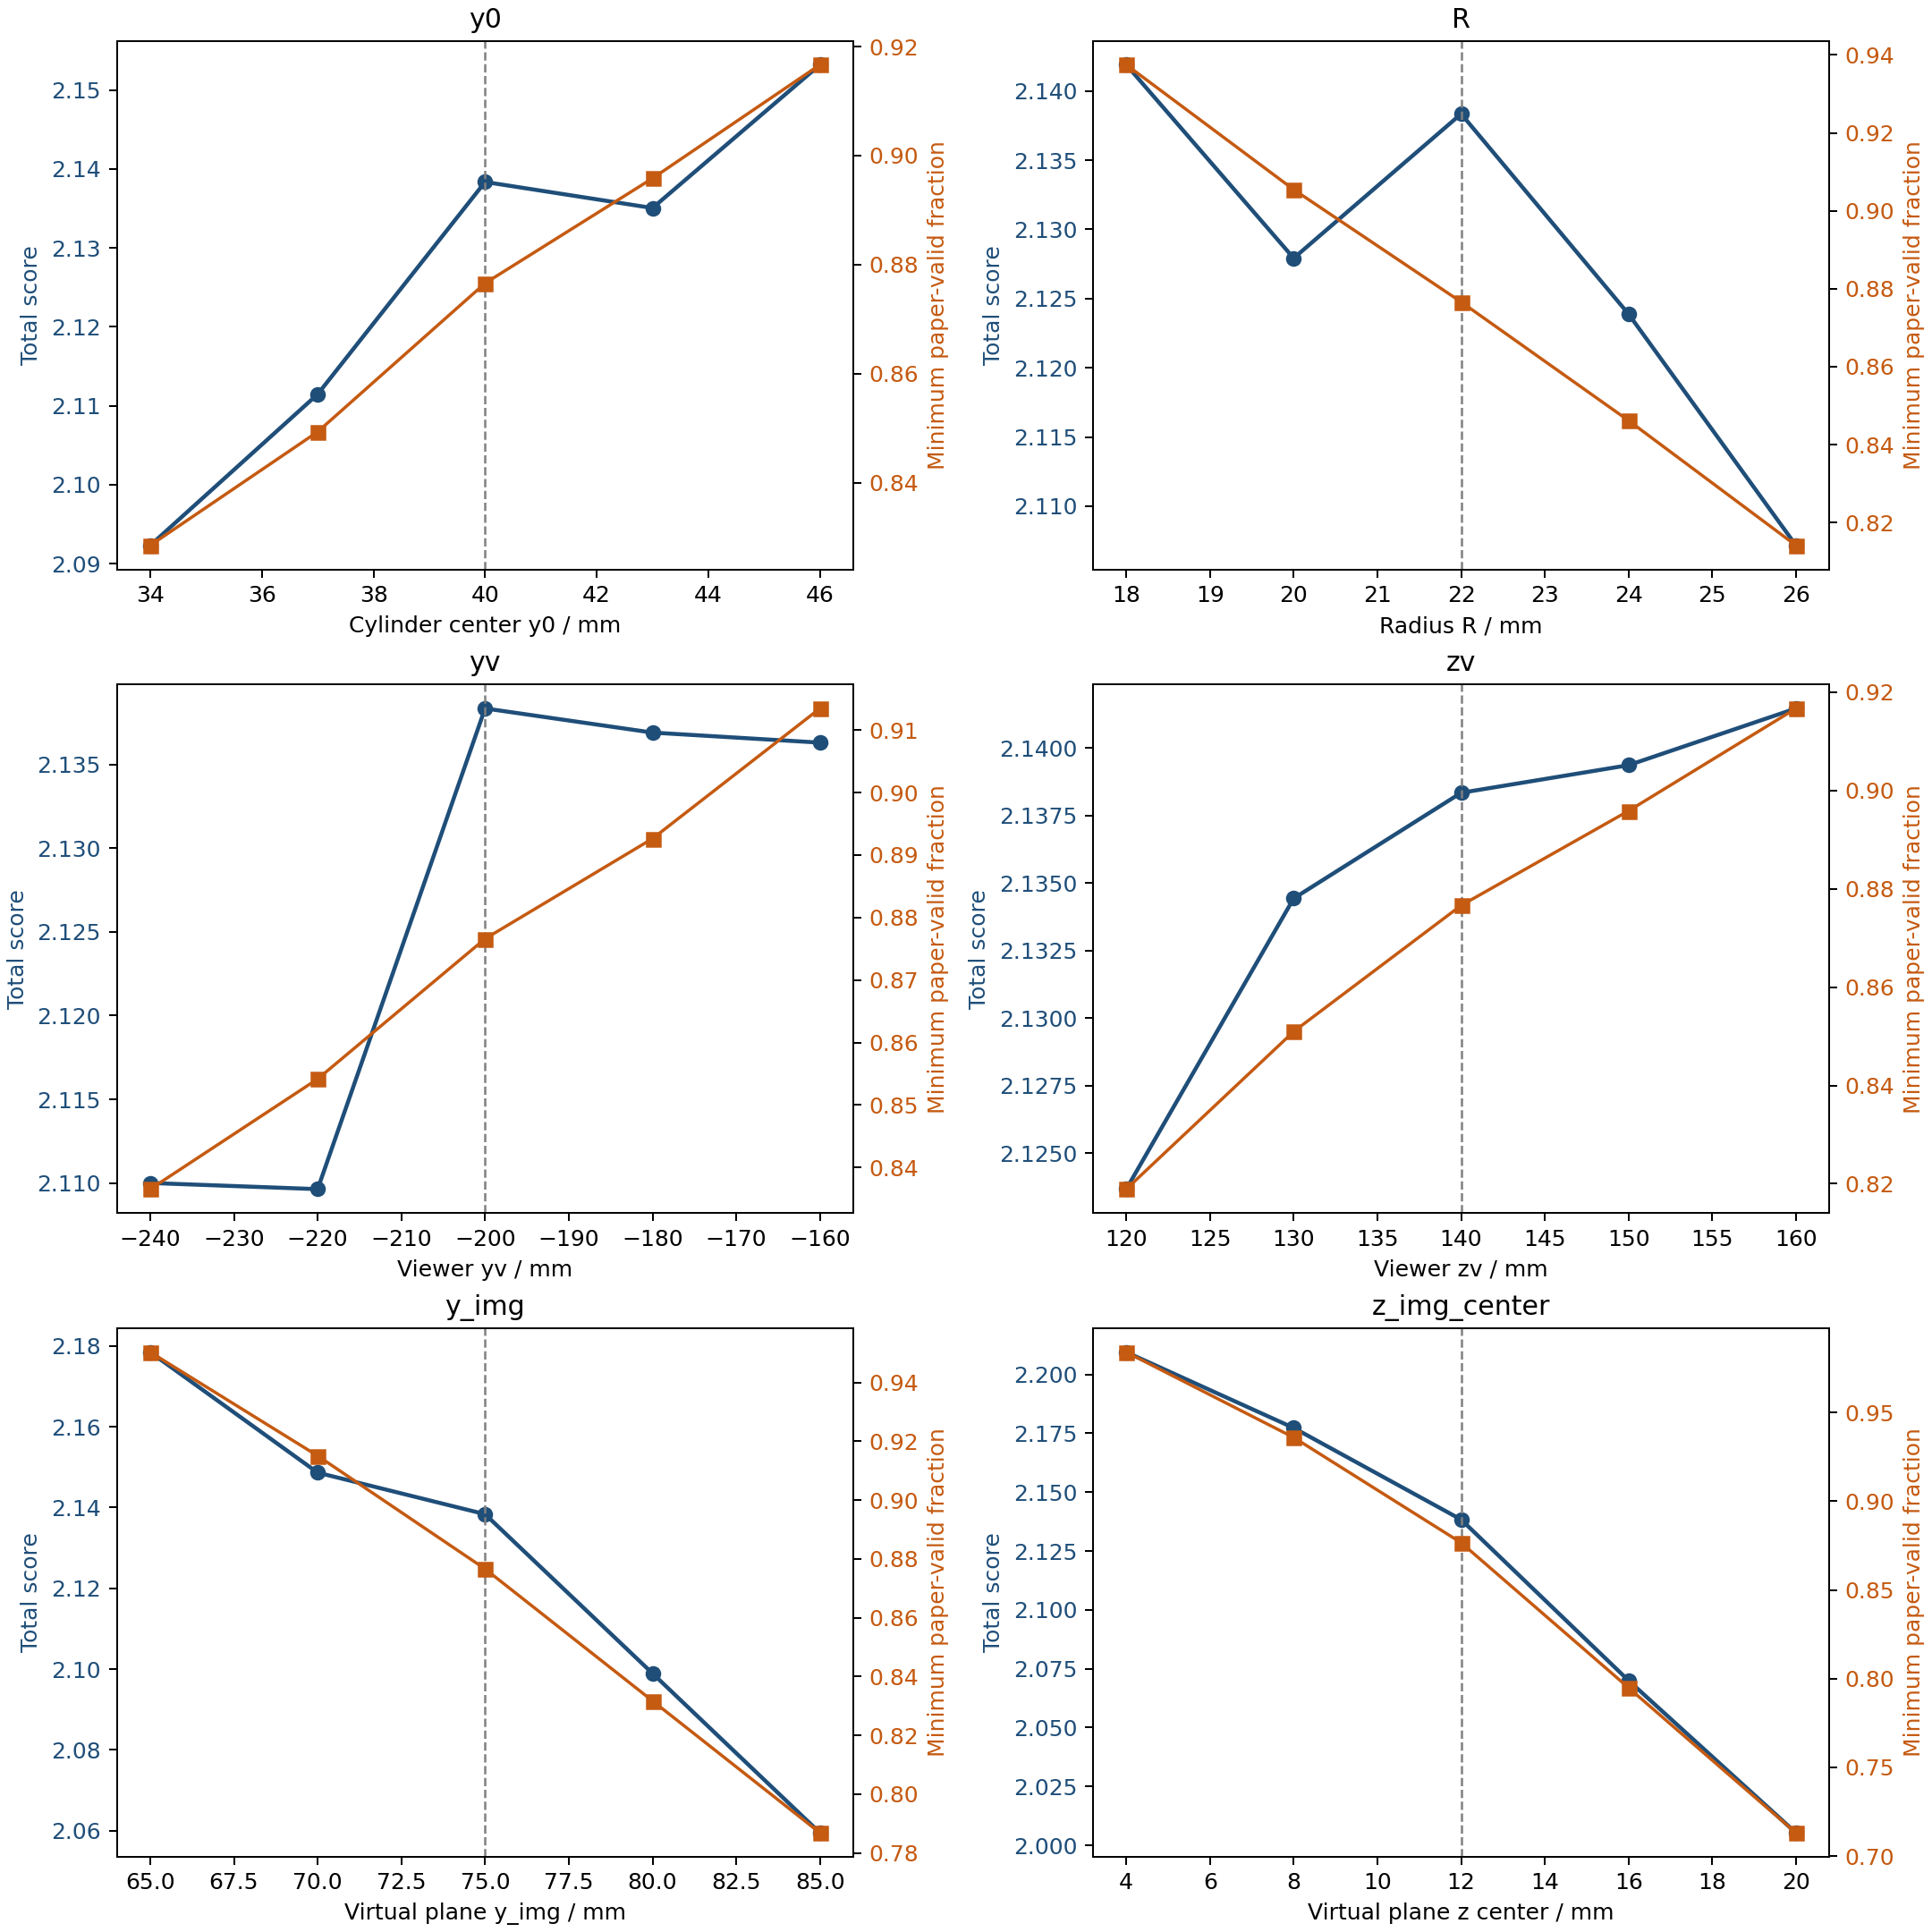
\includegraphics[width=0.85\textwidth]{../outputs/cylindrical_anamorphosis/sensitivity_score_and_coverage.png}
\caption{灵敏度分析：综合评分与纸张覆盖率}
\label{fig:sensitivity_score}
\end{figure}

图~\ref{fig:sensitivity_score}展示了关键参数变化对综合评分和纸张覆盖率的影响。从图中可以观察到：
\begin{itemize}
    \item 虚拟像平面位置$y_{img}$对结果影响显著，较低$y_{img}$值（靠近圆柱）可获得更高评分
    \item 虚拟像中心高度$z_{img\_center}$对覆盖率影响明显，较低高度有利于提高纸张利用率
    \item 圆柱半径$R$和观察点距离$y_v$在合理范围内变化时，模型表现相对稳定
\end{itemize}

\begin{figure}[H]
\centering
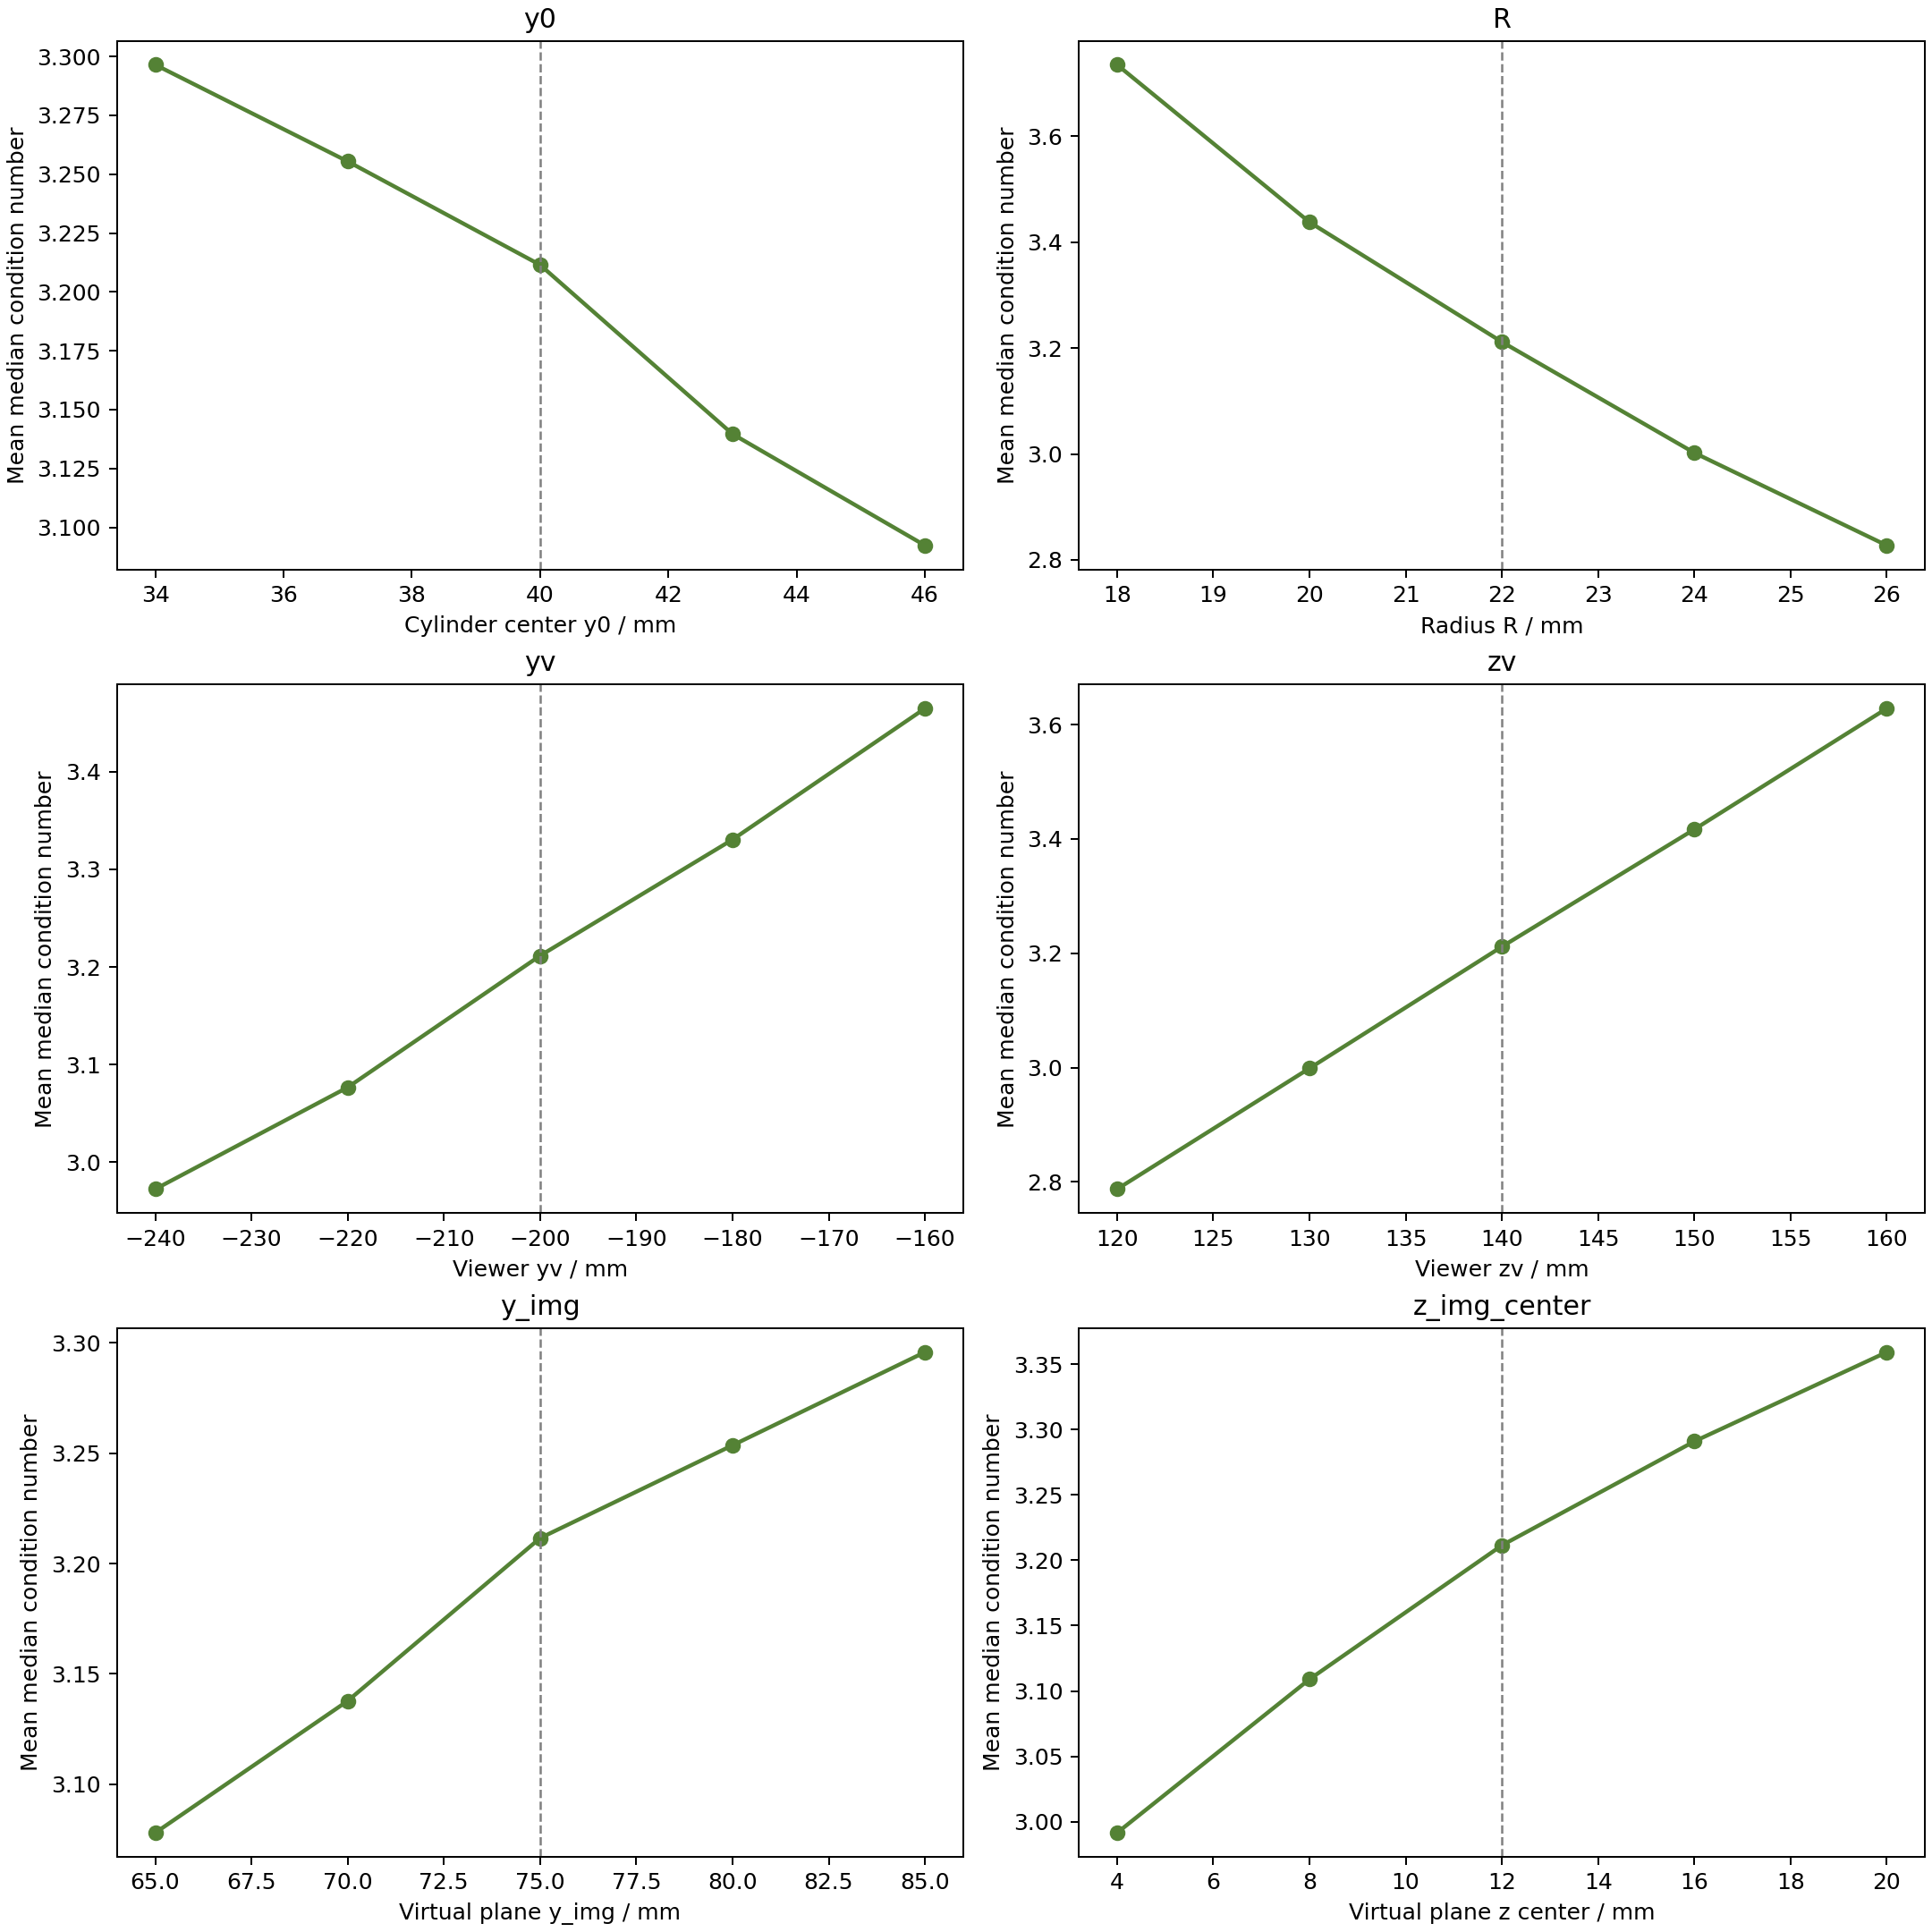
\includegraphics[width=0.85\textwidth]{../outputs/cylindrical_anamorphosis/sensitivity_condition_numbers.png}
\caption{灵敏度分析：Jacobian条件数分布}
\label{fig:sensitivity_cond}
\end{figure}

图~\ref{fig:sensitivity_cond}展示了不同参数配置下的Jacobian条件数分布。条件数反映了局部畸变程度，值越小表示畸变越均匀。分析表明，当前最优配置的条件数分布较为集中，大部分区域条件数小于4，满足可接受范围。

\subsection{灵敏度分析结论}

灵敏度分析结果表明：
\begin{enumerate}
    \item 模型对虚拟像平面位置$y_{img}$和中心高度$z_{img\_center}$较为敏感，这两个参数需要在优化过程中精细调整
    \item 圆柱半径$R$在20-24mm范围内变化时，模型表现相对稳定
    \item 观察点高度$z_v$对结果影响较小，在一定范围内可灵活调整
    \item 重建验证指标证实了模型的高精度和可靠性
\end{enumerate}

\section{模型评价与推广}

\subsection{模型优点}

\begin{enumerate}
    \item \textbf{物理基础严谨}：模型基于几何光学反射定律，建立了精确的逆反射链，数学推导严密
    \item \textbf{理论分析深入}：从拓扑、频率、几何三个维度建立了双图像相容性理论，给出了精确解不存在的严格证明
    \item \textbf{畸变度量完善}：采用Jacobian奇异值分解量化局部畸变，条件数指标具有明确几何意义
    \item \textbf{实用性强}：生成的变形图案满足A4约束，可直接用于实际制作
    \item \textbf{验证充分}：通过重建验证和灵敏度分析，证明了模型的正确性和稳定性
\end{enumerate}

\subsection{模型缺点}

\begin{enumerate}
    \item \textbf{理想化假设}：假设镜面为理想反射面，未考虑实际镜面的加工误差和反射损失
    \item \textbf{单视点限制}：模型基于单观察点，实际观察时人眼移动会导致图像畸变
    \item \textbf{计算复杂度}：Jacobian计算涉及数值微分，大规模图像处理时计算量较大
    \item \textbf{近似解依赖经验}：容忍畸变阈值的选择缺乏统一标准，依赖经验判断
\end{enumerate}

\subsection{模型改进方向}

\begin{enumerate}
    \item 引入镜面误差模型，分析加工精度对成像质量的影响
    \item 建立多视点优化模型，扩大清晰观察区域
    \item 开发GPU加速算法，提高大规模图像处理效率
    \item 研究基于人眼视觉特性的畸变容忍度量化方法
\end{enumerate}

\subsection{模型推广}

本文建立的逆反射链模型可推广至其他类型的变形艺术问题：
\begin{enumerate}
    \item \textbf{圆锥镜面变形}：将圆柱面替换为圆锥面，类似方法可推导逆反射链
    \item \textbf{球面镜面变形}：球面反射具有旋转对称性，可简化部分计算
    \item \textbf{多镜面系统}：扩展至多个镜面组合，建立更复杂的反射链
    \item \textbf{动态变形艺术}：引入时间维度，实现动画效果的变形显示
\end{enumerate}

\begin{thebibliography}{9}
\bibitem{1} 司守奎. 数学建模算法与应用[M]. 北京: 国防工业出版社, 2015.
\bibitem{2} 姜启源, 谢金星, 叶俊. 数学模型[M]. 北京: 高等教育出版社, 2011.
\bibitem{3} Hartley R, Zisserman A. Multiple View Geometry in Computer Vision[M]. Cambridge University Press, 2004.
\bibitem{4} 刘海洋. \LaTeX{}入门[M]. 北京: 电子工业出版社, 2013.
\bibitem{5} 华中杯数学建模竞赛组委会. 反射的艺术[B]. 2025.
\end{thebibliography}

\newpage
\begin{appendices}

\section{变形图案生成结果}

\begin{figure}[H]
\centering
\begin{minipage}[c]{0.48\textwidth}
\centering
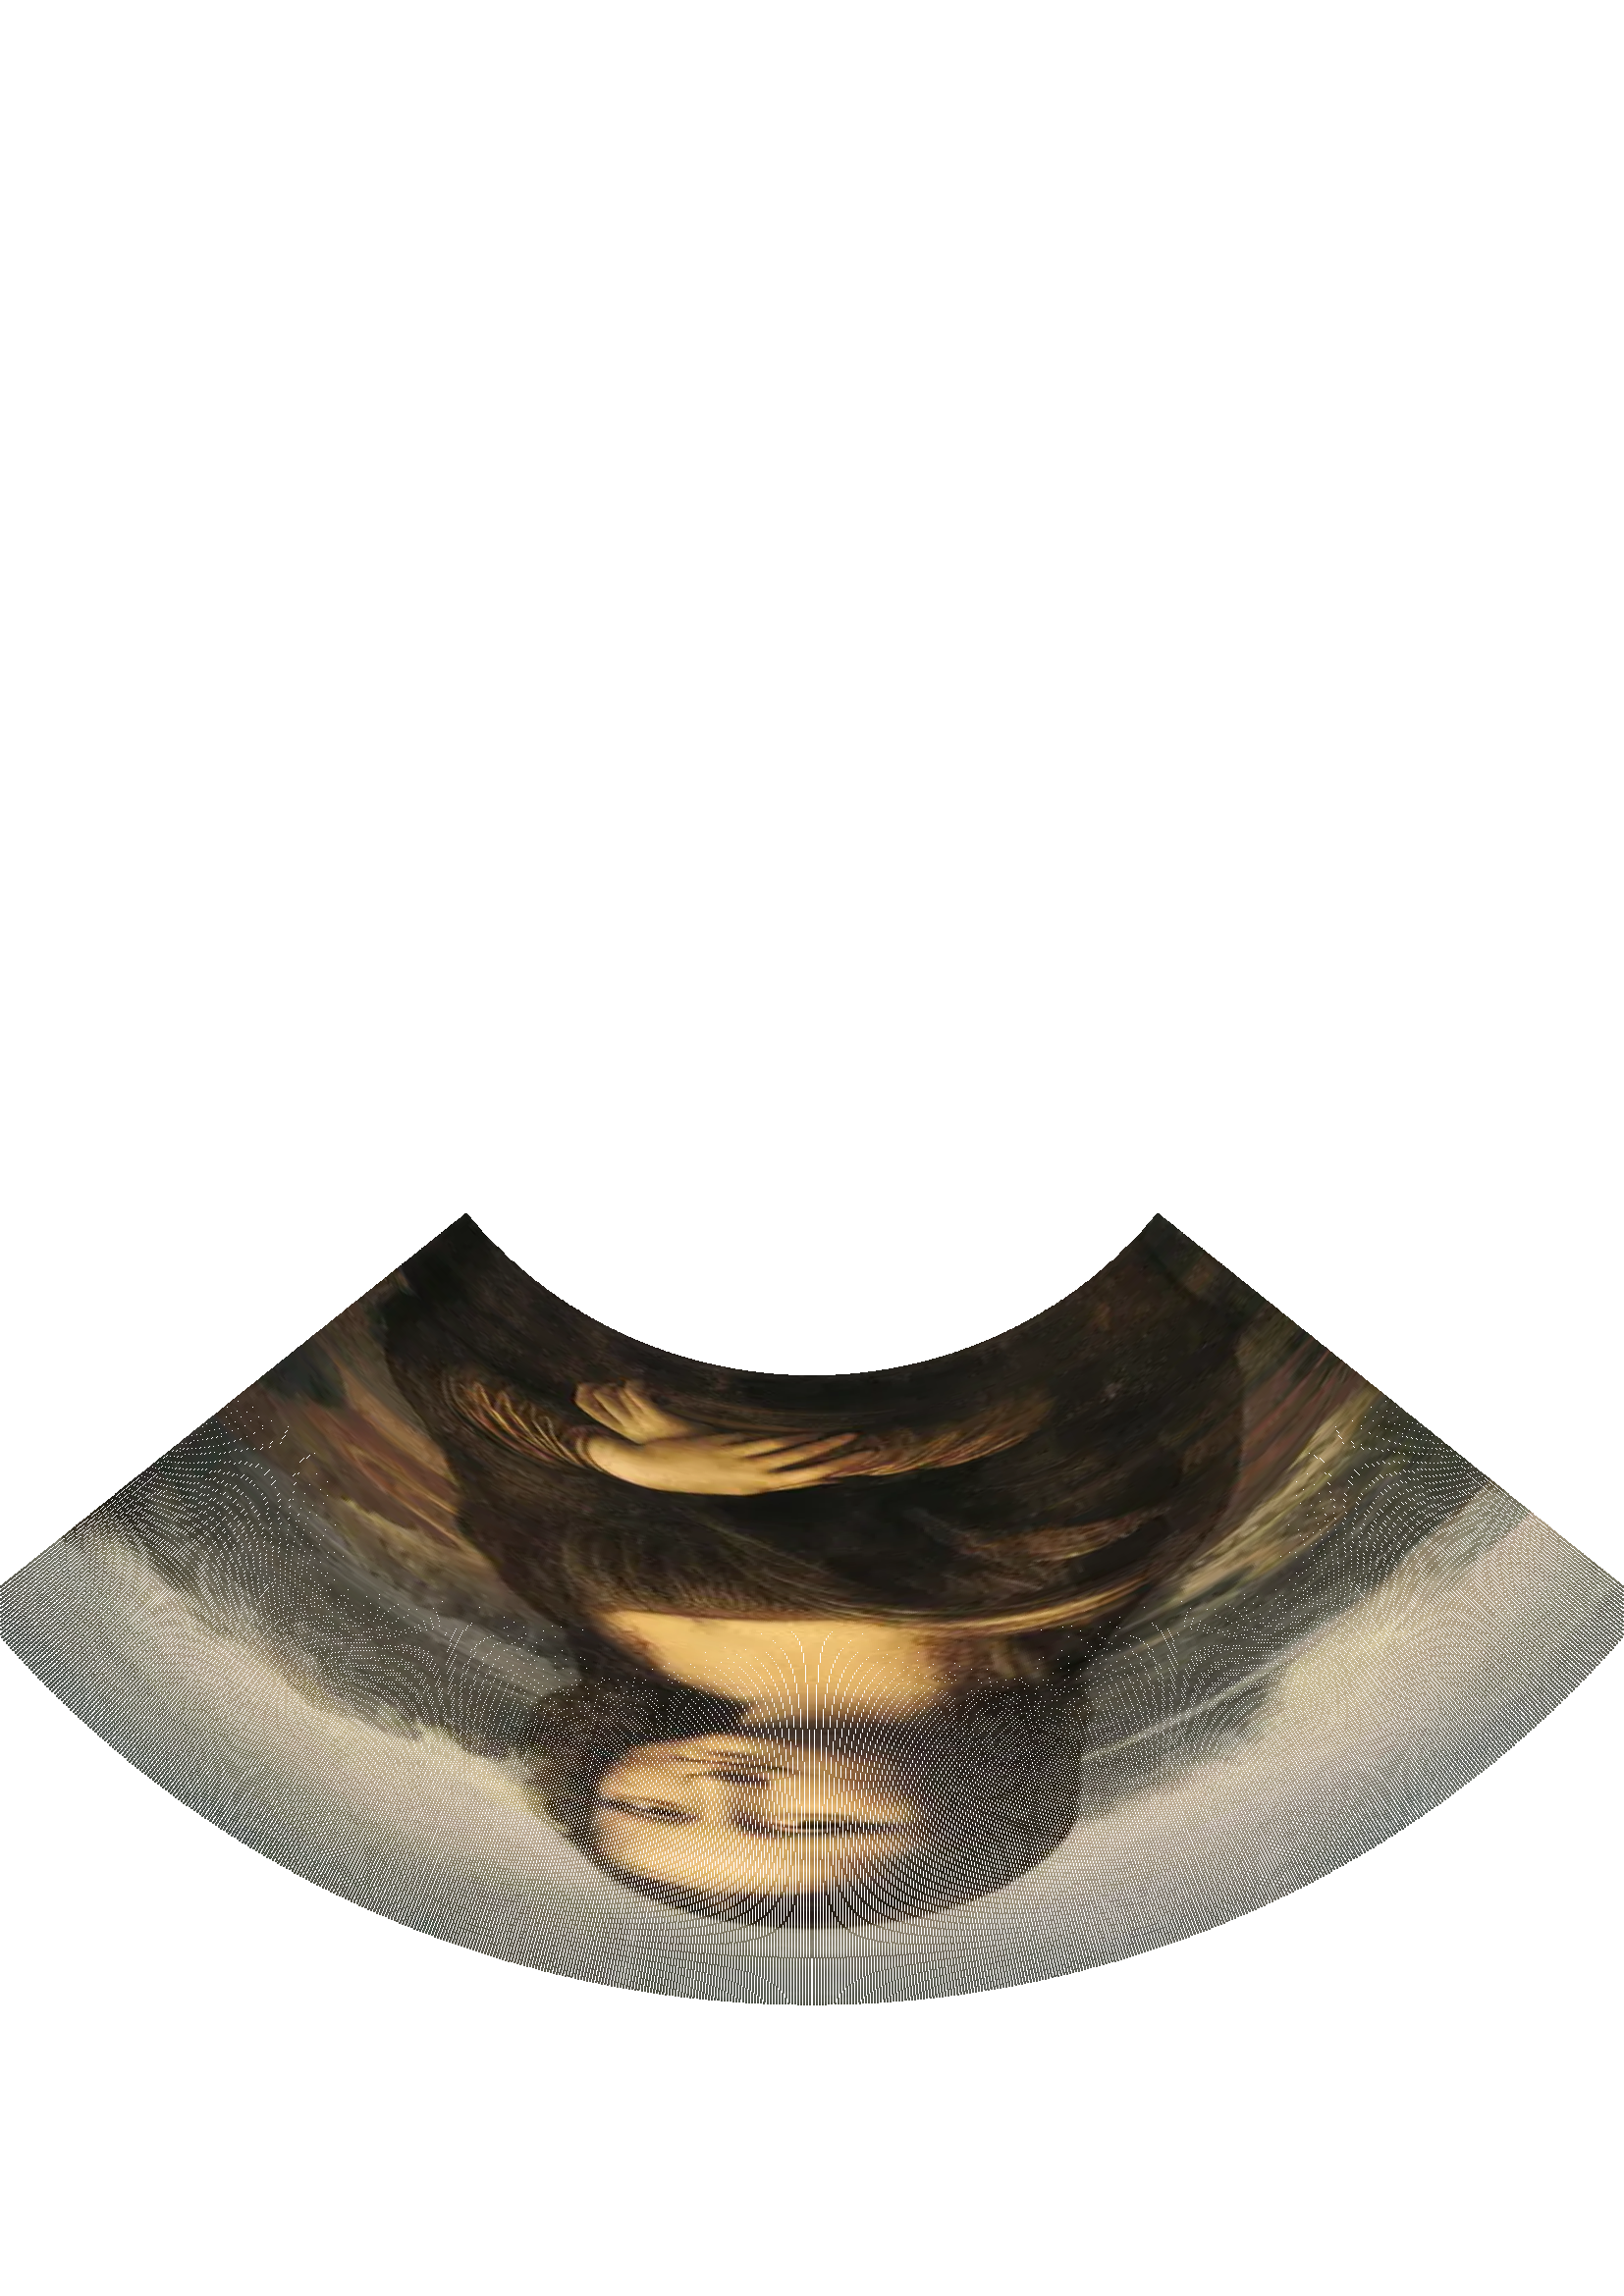
\includegraphics[width=0.95\textwidth]{../outputs/cylindrical_anamorphosis/fig3_paper_pattern.png}
\subcaption{图3变形图案}
\label{fig:fig3_pattern}
\end{minipage}
\begin{minipage}[c]{0.48\textwidth}
\centering
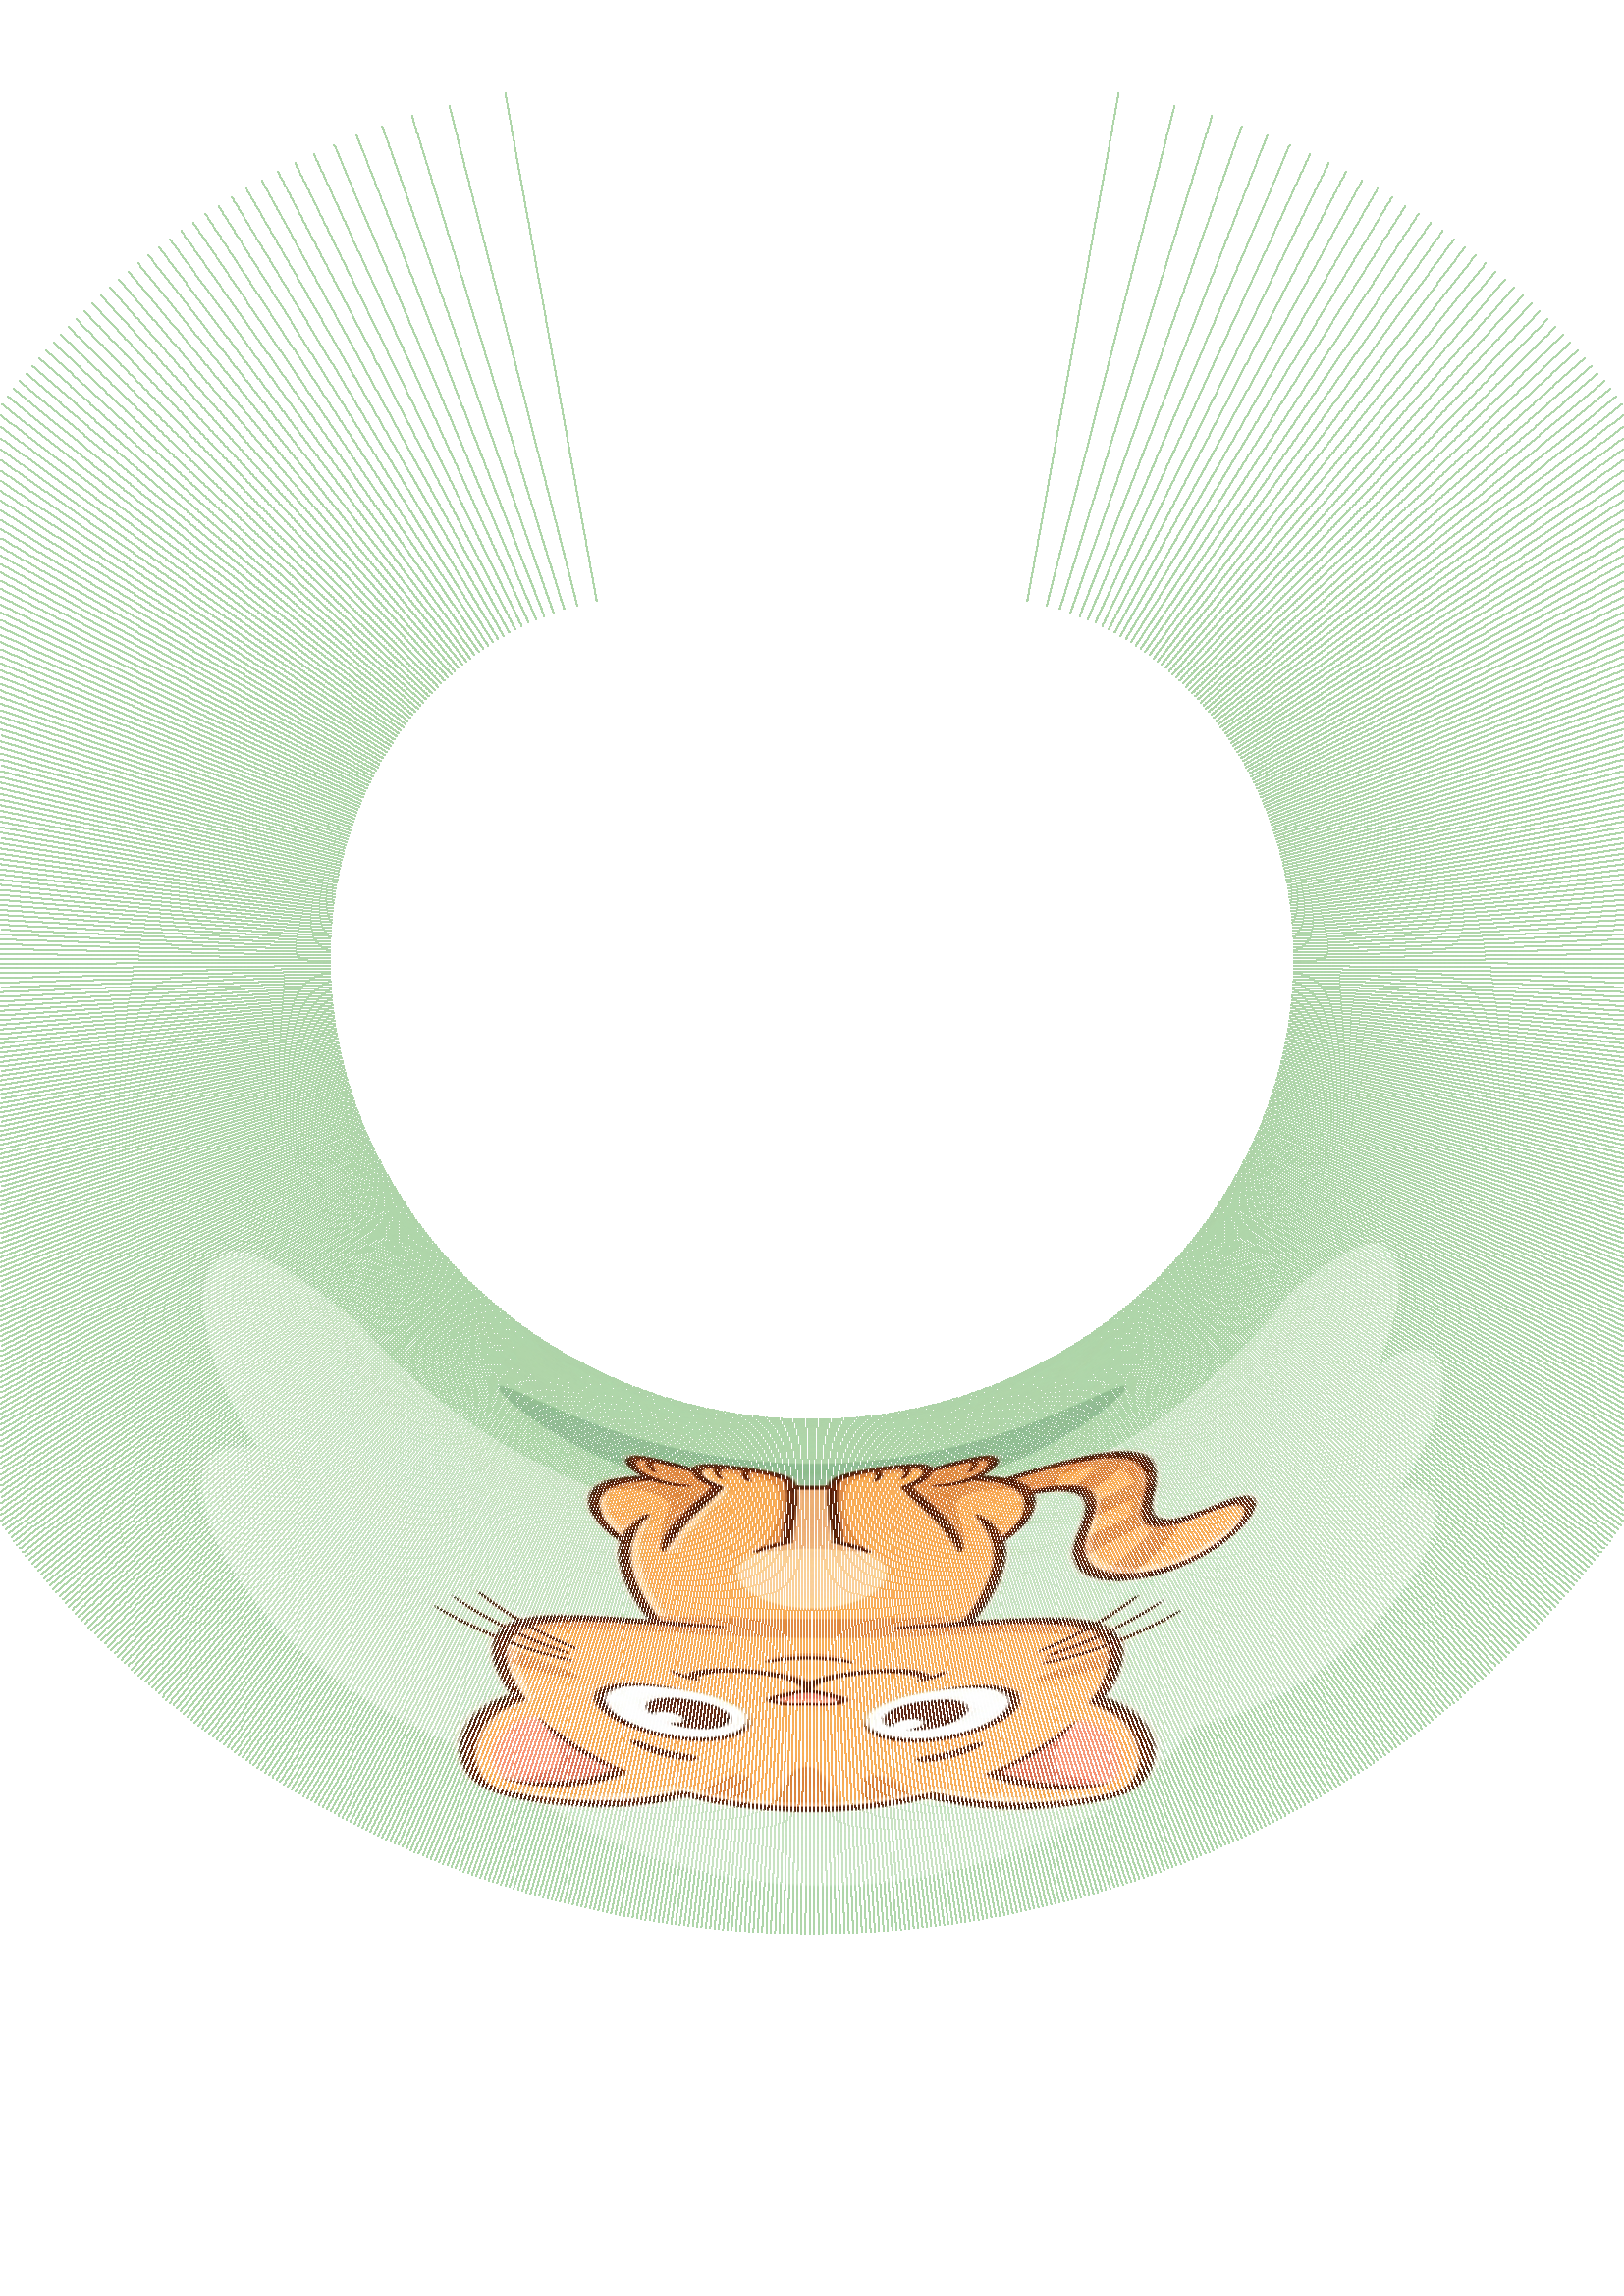
\includegraphics[width=0.95\textwidth]{../outputs/cylindrical_anamorphosis/fig4_paper_pattern.png}
\subcaption{图4变形图案}
\label{fig:fig4_pattern}
\end{minipage}
\caption{生成的变形图案}
\label{fig:patterns}
\end{figure}

\begin{figure}[H]
\centering
\begin{minipage}[c]{0.48\textwidth}
\centering
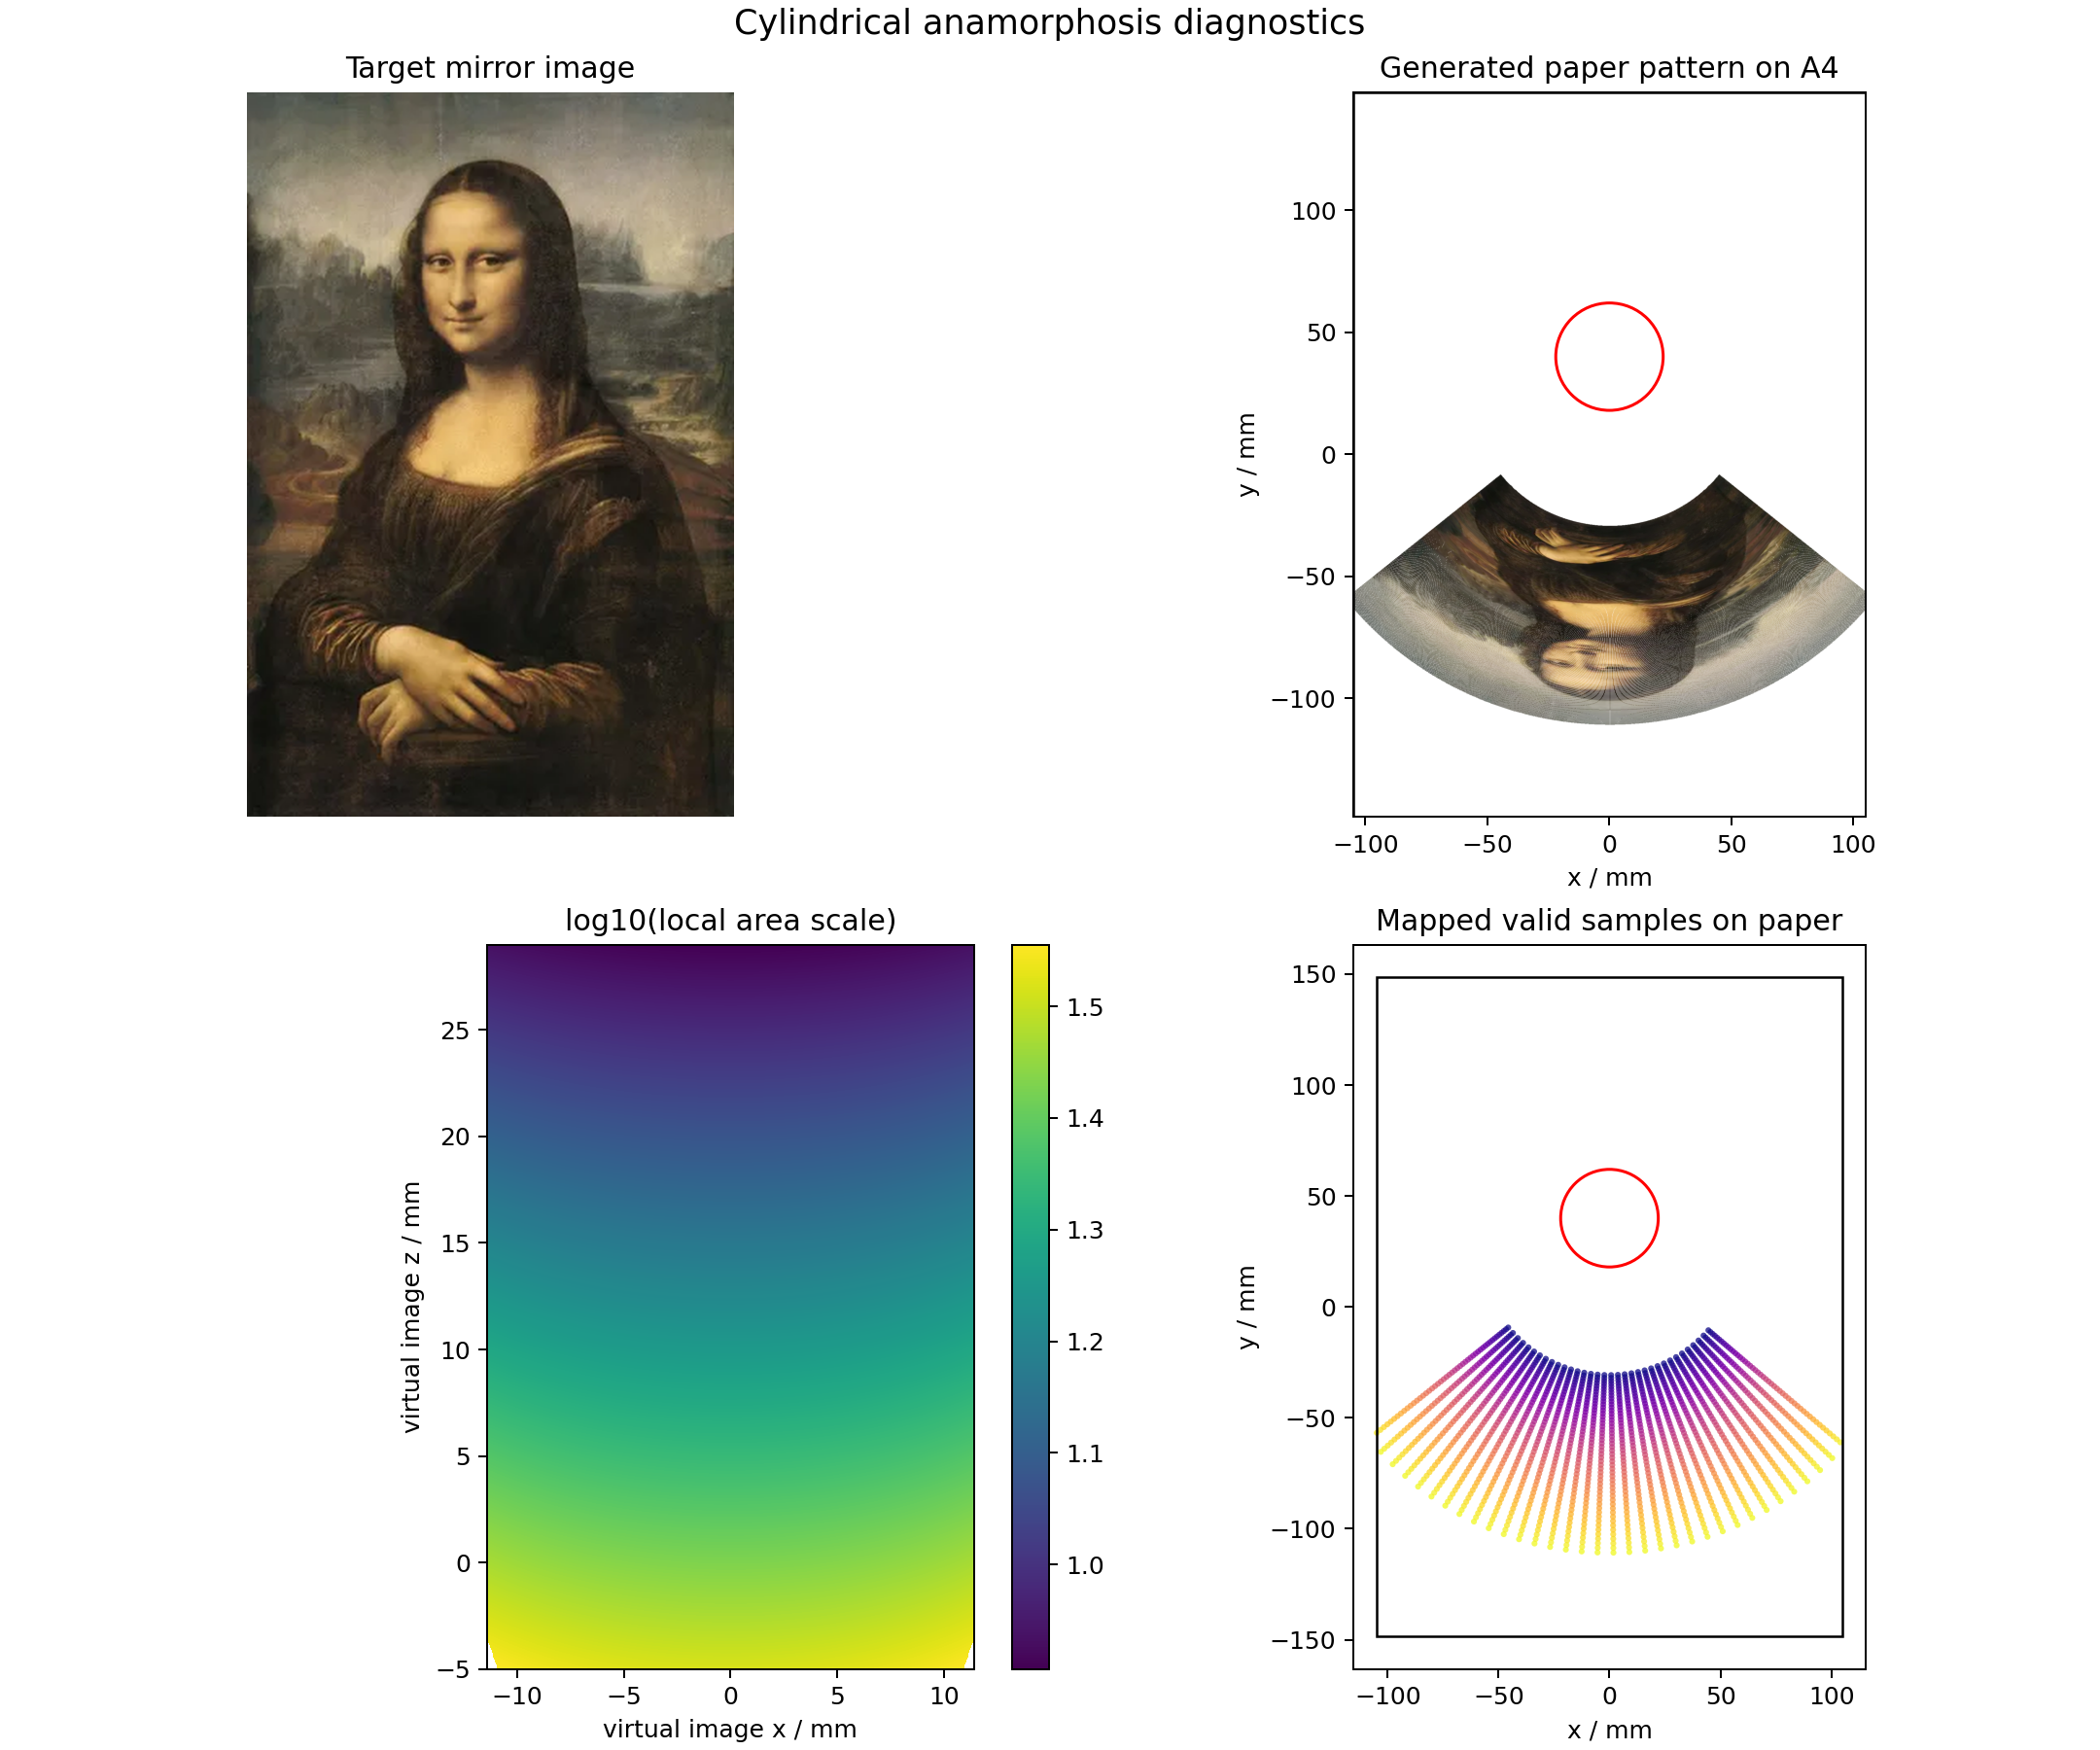
\includegraphics[width=0.95\textwidth]{../outputs/cylindrical_anamorphosis/fig3_diagnostic.png}
\subcaption{图3诊断图}
\label{fig:fig3_diag}
\end{minipage}
\begin{minipage}[c]{0.48\textwidth}
\centering
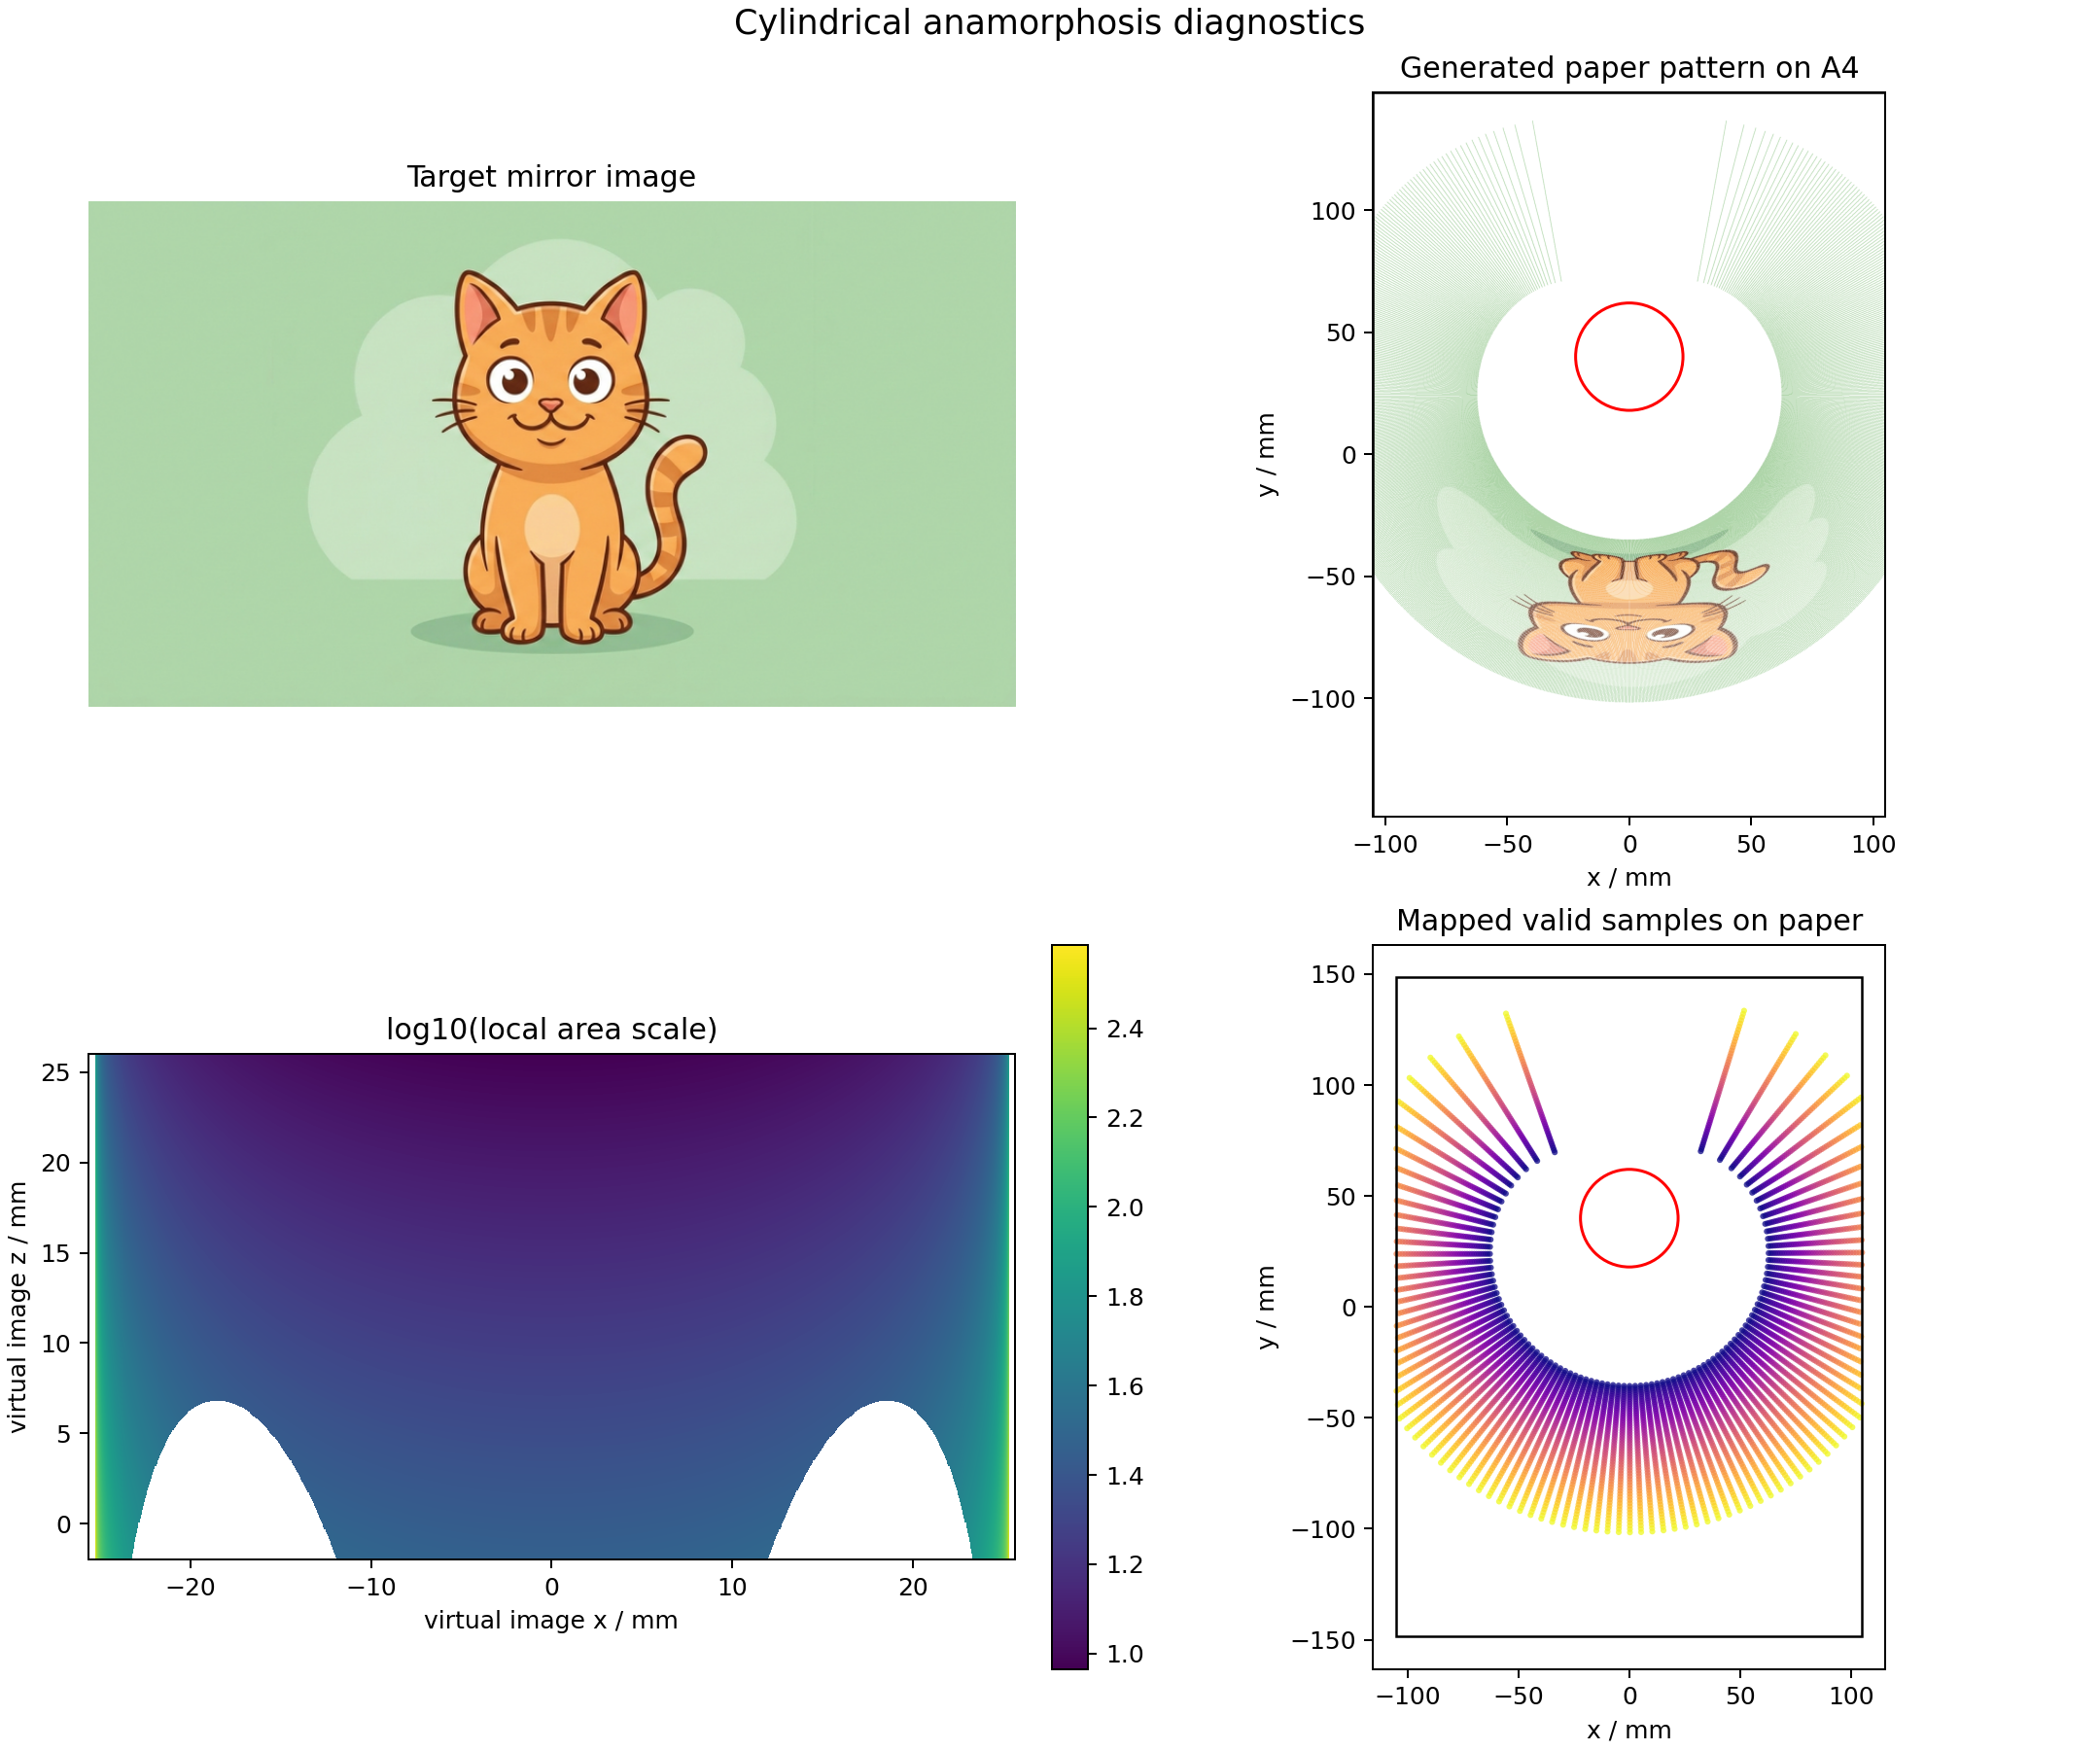
\includegraphics[width=0.95\textwidth]{../outputs/cylindrical_anamorphosis/fig4_diagnostic.png}
\subcaption{图4诊断图}
\label{fig:fig4_diag}
\end{minipage}
\caption{几何诊断可视化}
\label{fig:diagnostics}
\end{figure}

\begin{figure}[H]
\centering
\begin{minipage}[c]{0.48\textwidth}
\centering
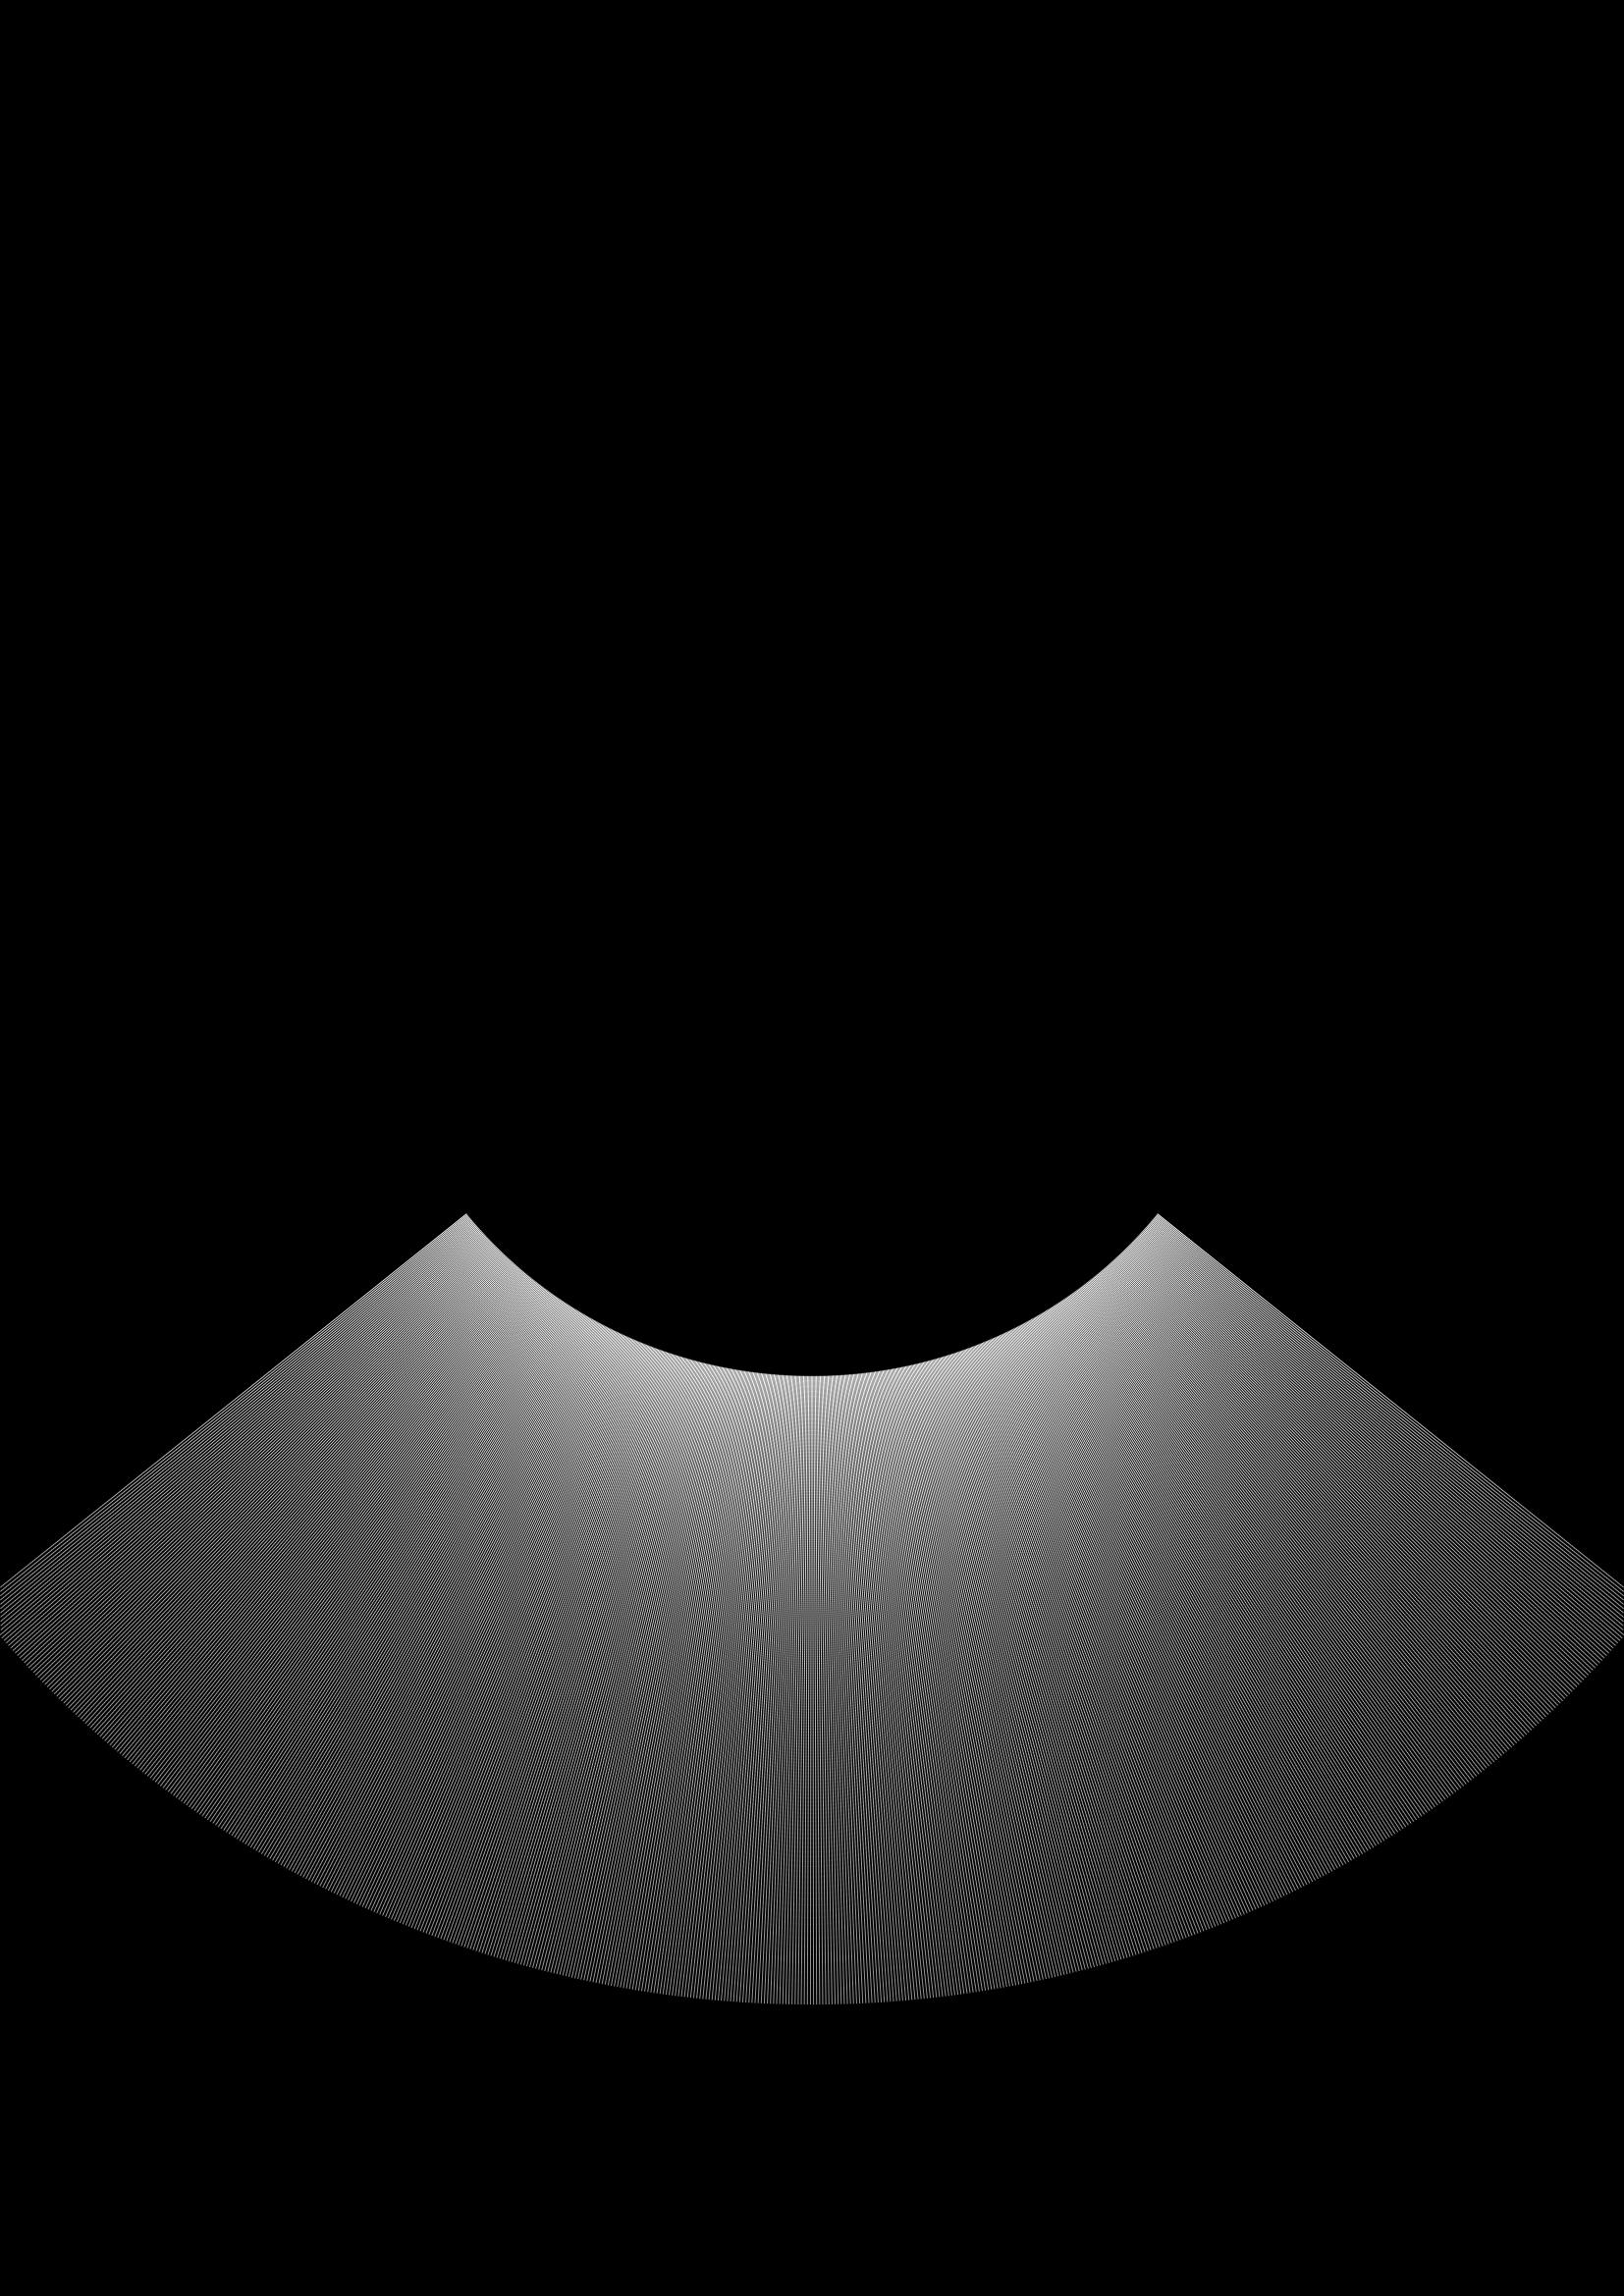
\includegraphics[width=0.95\textwidth]{../outputs/cylindrical_anamorphosis/fig3_occupancy.png}
\subcaption{图3纸张占用}
\label{fig:fig3_occ}
\end{minipage}
\begin{minipage}[c]{0.48\textwidth}
\centering
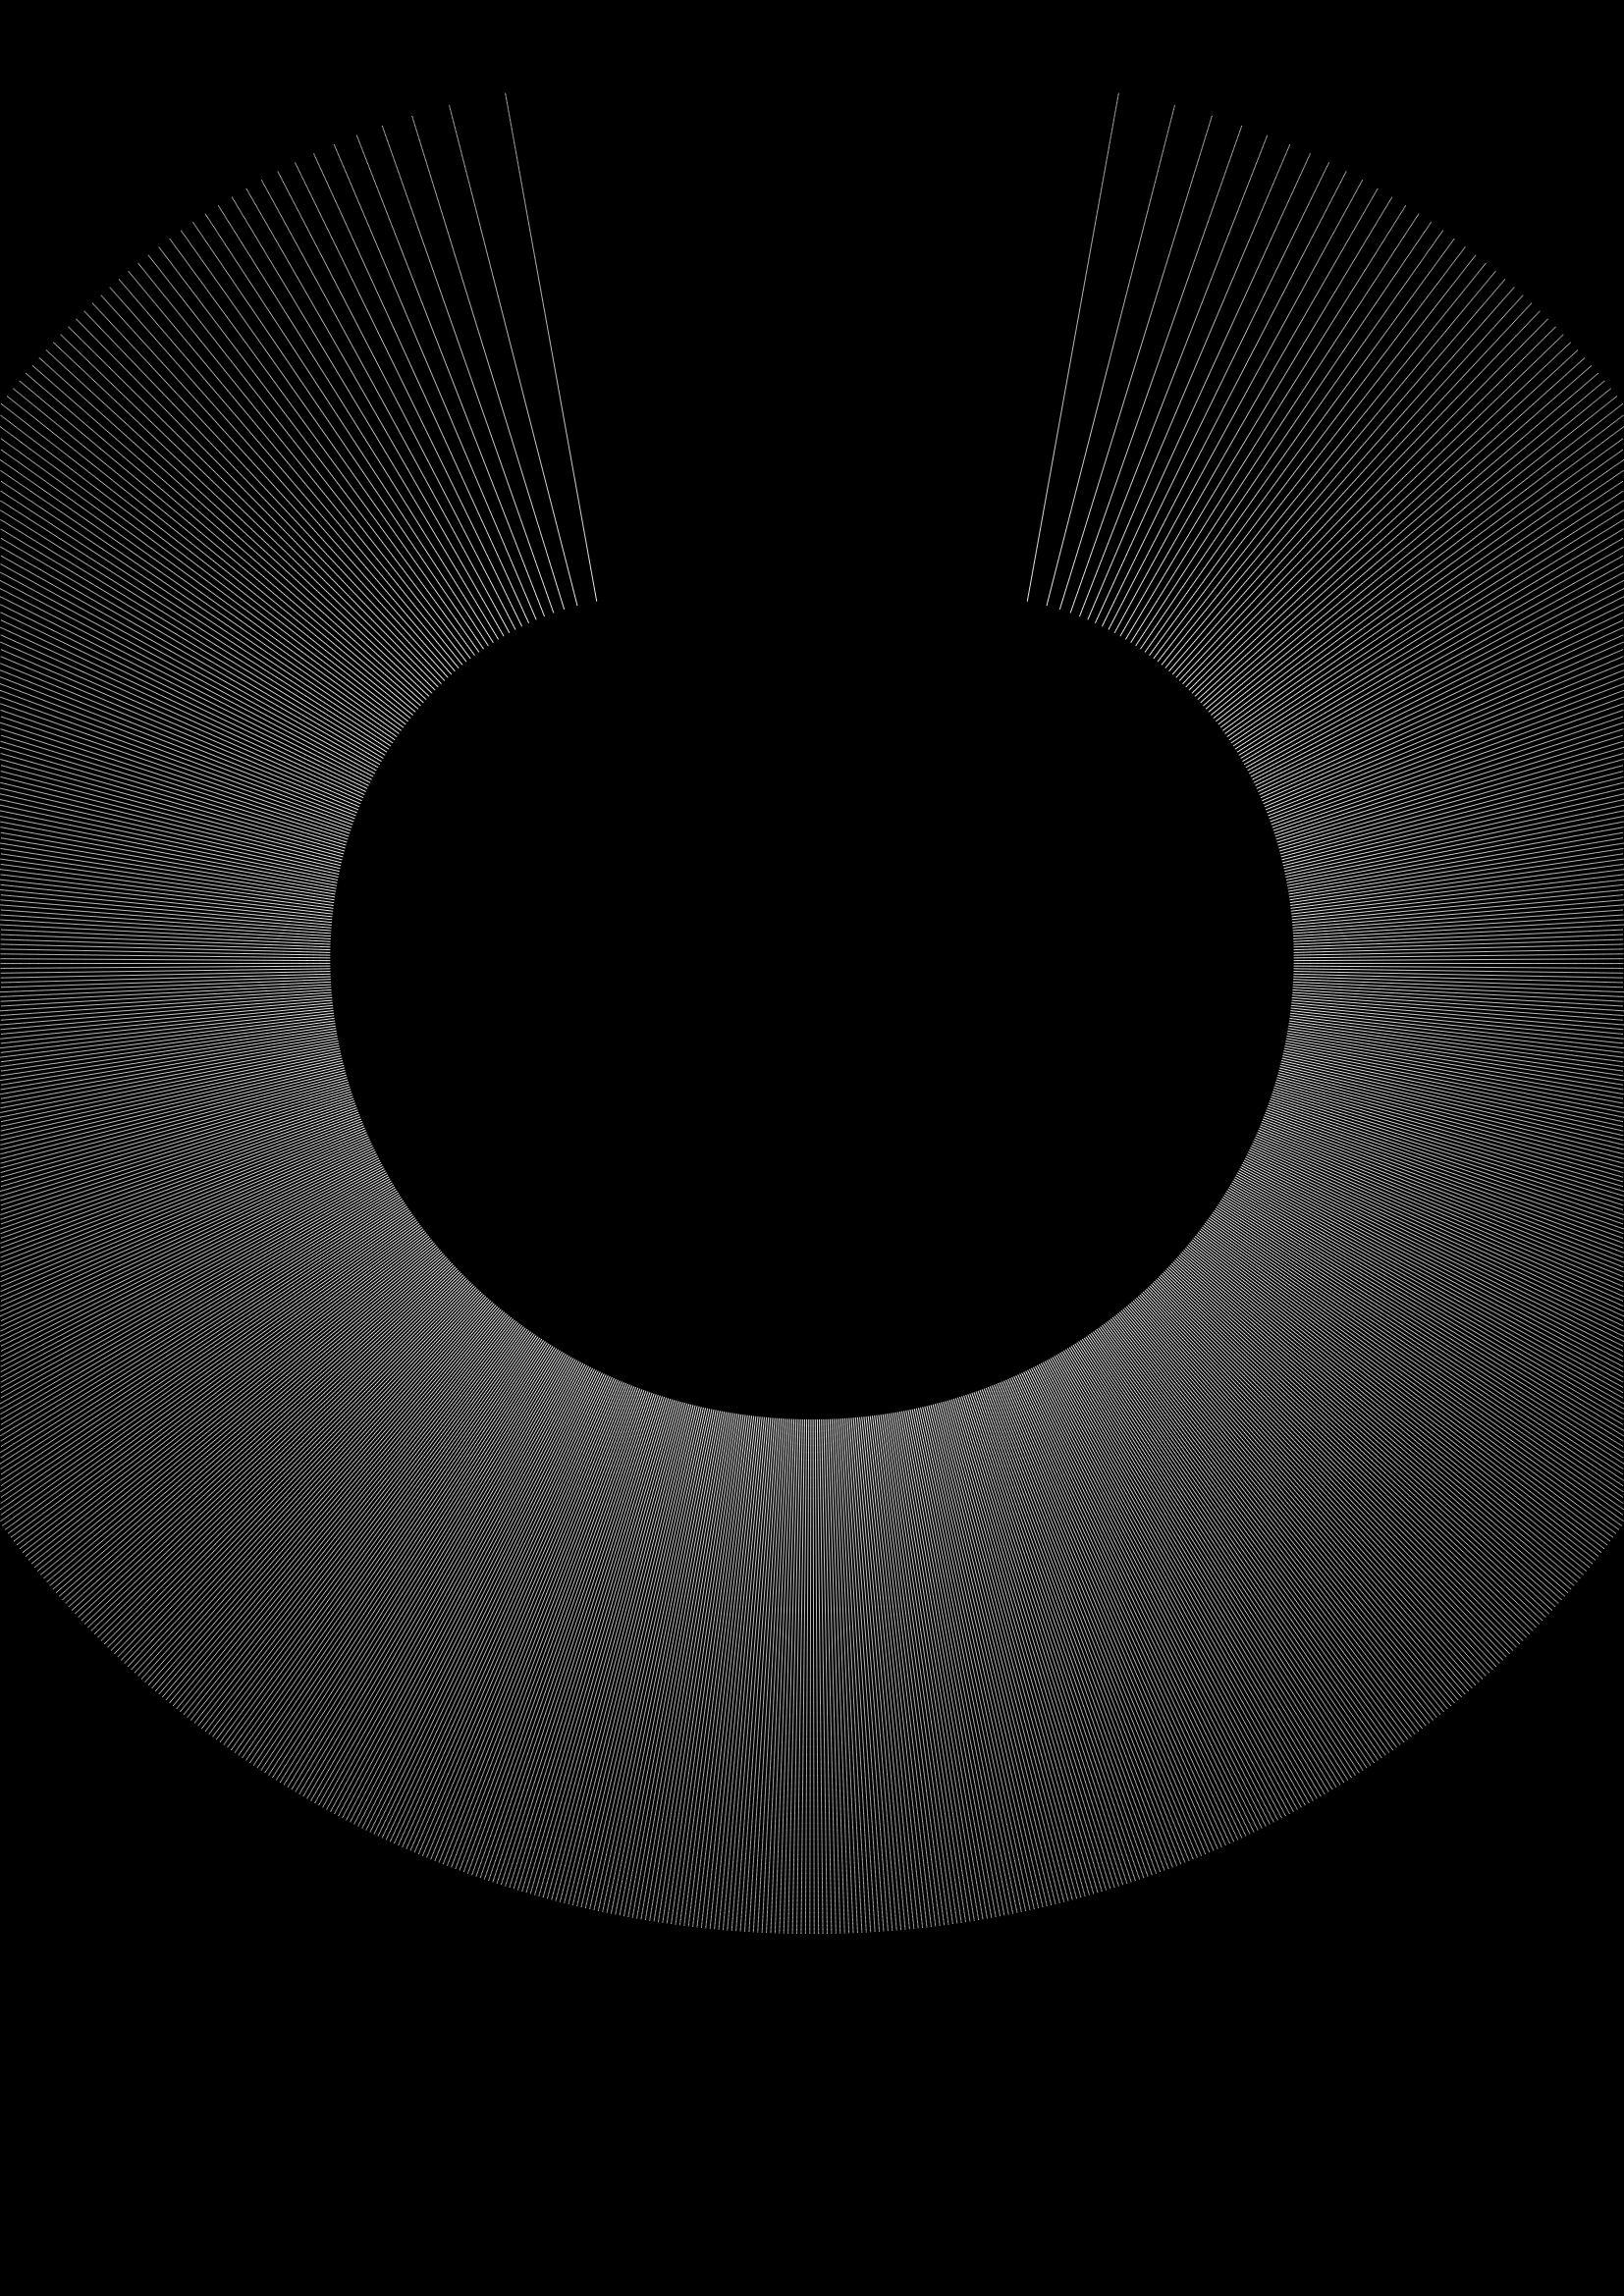
\includegraphics[width=0.95\textwidth]{../outputs/cylindrical_anamorphosis/fig4_occupancy.png}
\subcaption{图4纸张占用}
\label{fig:fig4_occ}
\end{minipage}
\caption{A4纸张占用分析}
\label{fig:occupancy}
\end{figure}

\section{核心算法伪代码}

\begin{lstlisting}[language=Python]
def inverse_reflection_chain(P_img, V, cylinder, paper_z=0):
    """
    逆反射链：从虚拟像点计算纸张图案点
    Parameters:
        P_img: 虚拟像点坐标 (x, y_img, z)
        V: 观察点坐标 (x_v, y_v, z_v)
        cylinder: 圆柱参数 (x0, y0, R, H)
    Returns:
        P_paper: 纸张上的图案点坐标
    """
    # Step 1: 视线与圆柱面求交
    d_view = P_img - V
    t = intersect_line_cylinder(V, d_view, cylinder)
    P_cyl = V + t * d_view
    
    # Step 2: 计算圆柱面法向量
    n = compute_cylinder_normal(P_cyl, cylinder)
    
    # Step 3: 应用反射定律
    d_out = normalize(P_img - P_cyl)
    d_in = d_out - 2 * dot(d_out, n) * n
    
    # Step 4: 求与纸张平面交点
    s = -P_cyl[2] / d_in[2]
    P_paper = P_cyl + s * d_in
    
    return P_paper

def compute_jacobian(P_img, theta, eps=1e-6):
    """计算映射的Jacobian矩阵"""
    J = zeros((2, 2))
    P0 = inverse_reflection_chain(P_img, V, cylinder)
    
    # 数值微分
    for i in range(2):
        P_perturb = P_img.copy()
        P_perturb[i] += eps
        P_perturbed = inverse_reflection_chain(P_perturb, V, cylinder)
        J[:, i] = (P_perturbed[:2] - P0[:2]) / eps
    
    return J
\end{lstlisting}

\section{Python实现代码}

\subsection{变形图案生成代码}

\lstinputlisting[language=Python, caption={generate\_patterns.py}]{../anamorphosis/generate_patterns.py}

\subsection{分析与可视化代码}

\lstinputlisting[language=Python, caption={generate\_analysis\_assets.py}]{../anamorphosis/generate_analysis_assets.py}

\end{appendices}

\end{document}
